\section{DẤU TAM THỨC BẬC HAI}
\subsection{TÓM TẮT LÝ THUYẾT}
\subsubsection{Tam thức bậc hai}
Tam thức bậc hai (đối với $x$) là biểu thức có dạng $f(x)=ax^2+bx+c$ $(a\neq 0)$.
\begin{boxkn}
	\begin{itemize}
		\item Khi thay $x=x_0$ thì $f(x_0)=ax_0^2+bx_0+c$ là giá trị của tam thức bậc hai tại $x_0$.
		\item Nghiệm của phương trình $ax^2+bx+c=0$ được gọi là nghiệm của tam thức bậc hai.
		\item $\Delta =b^2-4ac$ và $\Delta'=b'^2-ac$ theo thứ tự được gọi là biệt thức và biệt thức thu gọn của tam thức bậc hai.
	\end{itemize}
\end{boxkn}
\subsubsection{Định lý về dấu của tam thức bậc hai:}
Ta đã biết hàm số $y=ax^2+bx+c$ với $a \ne 0$ có đồ thị là một parabol.
\begin{itemize}
	\item [\iconCH] Nếu $a>0$, ta có các trường hợp sau\\
	\begin{minipage}{4cm}
		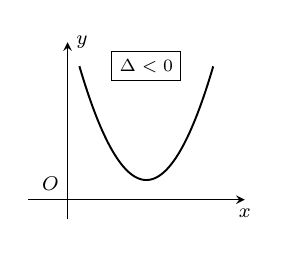
\begin{tikzpicture}[smooth,samples=300,scale=0.5,>=stealth,font=\footnotesize]
			\draw[->] (-1,0)--(4.5,0) node[below]{$x$};
			\draw[->] (0,-0.5)--(0,4) node[right]{$y$};
			\draw (0,0) node[above left]{$O$};
			\draw[line width=0.7pt,domain=0.3:3.7] plot(\x,{(\x)^2-4*(\x)+4.5});
			\node[below] at (2,4) {\fbox{\scriptsize$\Delta <0$}};
		\end{tikzpicture}\\
		\textbf{Đồ thị luôn nằm trên $Ox$.}
	\end{minipage}\hspace{1cm}
	\begin{minipage}{4cm}
		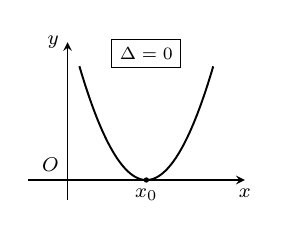
\begin{tikzpicture}[smooth,samples=300,scale=0.5,>=stealth,font=\footnotesize]
			\draw[->] (-1,0)--(4.5,0) node[below]{$x$};
			\draw[->] (0,-0.5)--(0,3.5) node[left]{$y$};
			\draw (0,0) node[above left]{$O$};
			\draw[line width=0.7pt,domain=0.3:3.7] plot(\x,{(\x)^2-4*(\x)+4});
			\draw[fill=black] (2,0) circle(1.5pt);
			\node[below] at (2,0) {$x_0$};
			\node[below] at (2,3.8) {\fbox{\scriptsize$\Delta =0$}};
		\end{tikzpicture}\\
		\textbf{Đồ thị nằm trên $Ox$ khi $x \ne x_0=-\frac{b}{2a}$.}
	\end{minipage}\hspace{1cm}
	\begin{minipage}{4cm}
		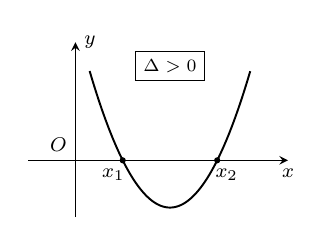
\begin{tikzpicture}[smooth,samples=300,scale=0.6,>=stealth,font=\footnotesize]
			\draw[->] (-1,0)--(4.5,0) node[below]{$x$};
			\draw[->] (0,-1.2)--(0,2.5) node[right]{$y$};
			\draw (0,0) node[above left]{$O$};
			\draw[line width=0.7pt,domain=0.3:3.7] plot(\x,{(\x)^2-4*(\x)+3});
			\draw[fill=black] (1,0) circle(1.5pt) (3,0) circle(1.5pt);
			\node[below] at (0.8,0) {$x_1$};
			\node[below] at (3.2,0) {$x_2$};
			\node[below] at (2,2.5) {\fbox{\scriptsize$\Delta >0$}};
		\end{tikzpicture}\\
		\textbf{Đồ thị nằm trên $Ox$ khi $x<x_1$ hoặc $x>x_2$; nằm dưới $Ox$ khi $x_1<x<x_2$.}
	\end{minipage}
	\item [\iconCH] Nếu $a<0$, ta có các trường hợp sau\\
	\begin{minipage}{4cm}
		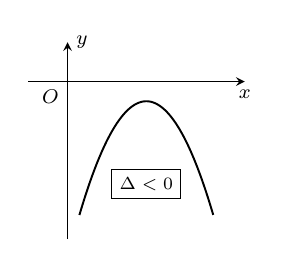
\begin{tikzpicture}[smooth,samples=300,scale=0.5,>=stealth,font=\footnotesize]
			\draw[->] (-1,0)--(4.5,0) node[below]{$x$};
			\draw[->] (0,-4)--(0,1) node[right]{$y$};
			\draw (0,0) node[below left]{$O$};
			\draw[line width=0.7pt,domain=0.3:3.7] plot(\x,{-(\x)^2+4*(\x)-4.5});
			\node[below] at (2,-2) {\fbox{\scriptsize$\Delta <0$}};
		\end{tikzpicture}\\
		\textbf{Đồ thị luôn nằm dưới $Ox$.}
	\end{minipage}\hspace{1cm}
	\begin{minipage}{4cm}
		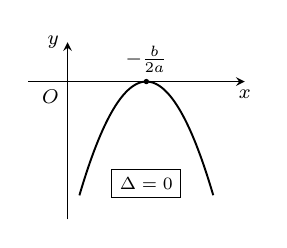
\begin{tikzpicture}[smooth,samples=300,scale=0.5,>=stealth,font=\footnotesize]
			\draw[->] (-1,0)--(4.5,0) node[below]{$x$};
			\draw[->] (0,-3.5)--(0,1) node[left]{$y$};
			\draw (0,0) node[below left]{$O$};
			\draw[line width=0.7pt,domain=0.3:3.7] plot(\x,{-(\x)^2+4*(\x)-4});
			\draw[fill=black] (2,0) circle(1.5pt);
			\node[above] at (2,0) {$-\frac{b}{2a}$};
			\node[below] at (2,-2) {\fbox{\scriptsize$\Delta =0$}};
		\end{tikzpicture}\\
		\textbf{Đồ thị nằm dưới $Ox$ khi $x \ne x_0=-\frac{b}{2a}$.}
	\end{minipage}\hspace{1cm}
	\begin{minipage}{4cm}
		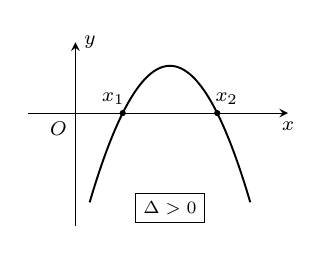
\begin{tikzpicture}[smooth,samples=300,scale=0.6,>=stealth,font=\footnotesize]
			\draw[->] (-1,0)--(4.5,0) node[below]{$x$};
			\draw[->] (0,-2.4)--(0,1.5) node[right]{$y$};
			\draw (0,0) node[below left]{$O$};
			\draw[line width=0.7pt,domain=0.3:3.7] plot(\x,{-(\x)^2+4*(\x)-3});
			\draw[fill=black] (1,0) circle(1.5pt) (3,0) circle(1.5pt);
			\node[above] at (0.8,0) {$x_1$};
			\node[above] at (3.2,0) {$x_2$};
			\node[below] at (2,-1.5) {\fbox{\scriptsize$\Delta >0$}};
		\end{tikzpicture}\\
		\textbf{Đồ thị nằm dưới $Ox$ khi $x<x_1$ hoặc $x>x_2$; nằm trên $Ox$ khi $x_1<x<x_2$.}
	\end{minipage}
\end{itemize}
Tương ứng hình ảnh đồ thị ở trên, ta có bảng tổng kết dấu của tam thức bậc hai như sau
\begin{itemize}
	\item [\iconCH] Nếu $a>0$:
	\begin{listEX}[3]
		\item [] 
\begin{tikzpicture}[scale=0.8,font=\footnotesize]
			\tkzTabInit[nocadre=false,lgt=1,espcl=2.5]
			{$x$ /0.6,$f(x)$ /0.6}
			{$-\infty$,$+\infty$}
			\tkzTabLine{,+,}
		\end{tikzpicture}
		\item [] 
\begin{tikzpicture}[scale=0.8,font=\footnotesize]
			\tkzTabInit[nocadre=false,lgt=1,espcl=1.4]
			{$x$ /0.6,$f(x)$ /0.6}
			{$-\infty$,$x_0$,$+\infty$}
			\tkzTabLine{,+,$0$,+,}
		\end{tikzpicture}
		\item [] 
\begin{tikzpicture}[scale=0.8,font=\footnotesize]
			\tkzTabInit[nocadre=false,lgt=1,espcl=1.2]
			{$x$ /0.6,$f(x)$ /0.6}
			{$-\infty$,$x_1$,$x_2$,$+\infty$}
			\tkzTabLine{,+,$0$,-,$0$,+,}
		\end{tikzpicture}
	\end{listEX}
	\item [\iconCH] Nếu $a<0$:
	\begin{listEX}[3]
		\item [] 
\begin{tikzpicture}[scale=0.8,font=\footnotesize]
			\tkzTabInit[nocadre=false,lgt=1,espcl=2.5]
			{$x$ /0.6,$f(x)$ /0.6}
			{$-\infty$,$+\infty$}
			\tkzTabLine{,-,}
		\end{tikzpicture}
		\item [] 
\begin{tikzpicture}[scale=0.8,font=\footnotesize]
			\tkzTabInit[nocadre=false,lgt=1,espcl=1.4]
			{$x$ /0.6,$f(x)$ /0.6}
			{$-\infty$,$x_0$,$+\infty$}
			\tkzTabLine{,-,$0$,-,}
		\end{tikzpicture}
		\item [] 
\begin{tikzpicture}[scale=0.8,font=\footnotesize]
			\tkzTabInit[nocadre=false,lgt=1,espcl=1.2]
			{$x$ /0.6,$f(x)$ /0.6}
			{$-\infty$,$x_1$,$x_2$,$+\infty$}
			\tkzTabLine{,-,$0$,+,$0$,-,}
		\end{tikzpicture}
	\end{listEX}
\end{itemize}

\begin{dl}[Định lý về dấu tam thức bậc hai]
	Cho tam thức bậc hai $f(x)=ax^2+b x+c$ $(a \neq 0)$.
	\begin{itemize}
		\item [\iconCH] Nếu $\Delta<0$ thì $f(x)$ cùng dấu với hệ số $a$ với mọi $x \in \mathbb{R}$.
		\item [\iconCH] Nếu $\Delta=0$ thì $f(x)$ cùng dấu với hệ số $a$ với mọi $x \neq-\dfrac{b}{2a}$.
		\item [\iconCH] Nếu $\Delta>0$ thì tam thức $f(x)$ có hai nghiệm phân biệt $x_1$ và $x_2$ $\left(x_{1}<x_{2}\right)$. Khi đó, $f(x)$ cùng dấu với hệ số $a$ với mọi $x \in\left(-\infty ; x_{1}\right) \cup\left(x_{2} ;+\infty\right) ; f(x)$ trái dấu với hệ số $a$ với mọi $x \in\left(x_{1} ; x_{2}\right)$.
	\end{itemize}
\end{dl}

\begin{khung4}{Ghi nhớ dấu của $f(x)$ và $a$}
	\begin{itemize}
		\item[\iconCH] Nếu $\Delta < 0$ thì
		\begin{center}
			\begin{tikzpicture}
				\tkzTabInit[nocadre=false,lgt=1.2,espcl=4.2]
				{$x$ /0.7,$f(x)$ /0.8}
				{$-\infty$,$+\infty$}
				\tkzTabLine{,\text{cùng dấu $a$},}
			\end{tikzpicture}
		\end{center}
		\item[\iconCH] Nếu $\Delta = 0$ thì
		\begin{center}
			\begin{tikzpicture}
				\tkzTabInit[nocadre=false,lgt=1.2,espcl=3]
				{$x$ /0.7,$f(x)$ /0.8}
				{$-\infty$,$-\frac{b}{2a}$,$+\infty$}
				\tkzTabLine{,\text{cùng dấu $a$},$0$,\text{ cùng dấu $a$},}
			\end{tikzpicture}
		\end{center}
		\item[\iconCH] Nếu $\Delta > 0$ thì
		\begin{center}
			\begin{tikzpicture}
				\tkzTabInit[nocadre=false,lgt=1.2,espcl=3]
				{$x$ /0.7,$f(x)$ /1}
				{$-\infty$,$x_1$,$x_2$,$+\infty$}
				\tkzTabLine{,\text{\textbf{cùng} dấu $a$},$0$,\text{ \textbf{trái} dấu $a$ },$0$,\text{ \textbf{cùng} dấu $a$},}
			\end{tikzpicture}
		\end{center}
		\textbf{Câu nhớ:} \lq\lq trong trái, ngoài cùng\rq\rq.
	\end{itemize}
\end{khung4}

\subsection{PHÂN LOẠI VÀ PHƯƠNG PHÁP GIẢI TOÁN}
\begin{dang}{Nhận diện và tìm điều kiện để một biểu thức là tam thức bậc hai}
	 Tam thức bậc hai (đối với $x$) là biểu thức có dạng $f(x)=ax^2+bx+c$ $(a\neq 0)$.\\
	 \textbf{Chú ý 1}\\
	 Nếu phương trình $a x^{2}+b x+c=0$ (và đặt $b'=\dfrac{b}{2}$) có
	 \begin{itemize}
	 	\item $\Delta<0$ (hoặc $\Delta'<0$) thì phương trình bậc hai đó vô nghiệm.
	 	\item $\Delta=0$ (hoặc $\left.\Delta^{\prime}=0\right)$ thì phương trình bậc hai đó có một nghiệm duy nhất $x=-\dfrac{b}{2 a}$ (hoặc $x=-\dfrac{b'}{a}$).
	 	\item $\Delta>0$ (hoặc $\Delta'>0$) thì phương trình bậc hai đó có hai nghiệm phân biệt $x=\dfrac{-b \pm \sqrt{\Delta}}{2 a}$ (hoặc $x=\dfrac{-b' \pm \sqrt{\Delta'}}{a}$).
	 \end{itemize}
\end{dang}

%%=====Ví dụ 1
\begin{vd}%[0D7N1-1]%[Dự án đề cương 3 khối NH24-25 - Đợt 1 - Quan Ón]
	Biểu thức nào sau đây là tam thức bậc hai? Nếu là tam thức bậc hai, hãy xét dấu của nó tại $x=1$.
	\begin{multicols}{3}
		\begin{enumerate}
			\item $f(x)=2x^2+x-1$.
			\item $g(x)=-x^4+2x^2+1$.
			\item $h(x)=-x^2+\sqrt{2}x-3$.
		\end{enumerate}
	\end{multicols}
	\loigiai{
		\begin{enumerate}
			\item Ta có $f(x)=2x^2+x-1$ là tam thức bậc hai.\\
			Với $x=1$ ta có $f(1)=2 \cdot 1^2+1-1=2 > 0$.
			\item Ta có $g(x)=-x^4+2x^2+1$ không là tam thức bậc hai.
			\item Ta có $h(x)=-x^2+\sqrt{2}x-3$ là tam thức bậc hai.\\
			Với $x=1$ ta có $h(1)=-1^2+\sqrt{2}\cdot 1-3=-4+\sqrt{2}<0$.
		\end{enumerate}
	}
\end{vd}

\begin{vd}%[0D7H1-1]%[Dự án đề cương 3 khối NH24-25 - Đợt 1 - Quan Ón]
	Tìm các giá trị của tham số $m$ để
	\begin{enumerate}
		\item $f(x) = (2m-8)x^2 + 2mx + 1$ là một tam thức bậc hai.
		\item $f(x) = mx^3 + (m-1)x^2 + 2mx + 1$ là một tam thức bậc hai.
		\item $f(x)= 2x^2 + 2mx + m^2 - 4m + 6$ là một tam thức bậc hai.
		\item $f(x) = 2x^2 + mx - 3$ dương tại $x=2$.
		\item $f(x)=x^2+3mx-3m+7$ âm tại $x=-1$.
	\end{enumerate}
	\loigiai{
		\begin{enumerate}
			\item Để $f(x)=(2m-8)x^2+2mx+1$ là một tam thức bậc hai thì $2m-8 \ne 0 \Leftrightarrow m \ne 4$.
			\item Để $f(x) = mx^3 + (m-1)x^2 + 2mx + 1$ là một tam thức bậc hai thì $\heva{&m=0\\&m-1\neq 0} \Leftrightarrow \heva{&m=0\\&m\neq 1} \Leftrightarrow m = 0$.
			\item $f(x)= 2x^2 + 2mx + m^2 - 4m + 6$ có $a = 2 \neq 0$, $\forall m \in \mathbb{R}$.\\
			Do đó $f(x)= 2x^2 + 2mx + m^2 - 4m + 6$ luôn là một tam thức bậc hai với mọi $m$.
			\item $f(x) = 2x^2 + mx - 3$ dương tại $x=2$ thì $f(2)>0$.\\
			Suy ra $f(2) = 2\cdot 2^2 + m\cdot 2 - 3 > 0 \Leftrightarrow 5-2m > 0 \Leftrightarrow  m <\dfrac{5}{2}$.
			\item $f(x)=x^2+3mx-3m+7$ âm tại $x=-1$ thì $f(-1)<0$.\\
			Suy ra $f(-1)= \left(-1 \right)^2  + 3m\cdot (-1) - 3m + 7 < 0 \Leftrightarrow -6m + 8 < 0 \Leftrightarrow m >\dfrac{4}{3}$.
		\end{enumerate}
	}
\end{vd}

\begin{vd}%%[0D7H1-1]%[Dự án đề cương 3 khối NH24-25 - Đợt 1 - Quan Ón]
	Tìm các giá trị của tham số $m$ để $f(x)=(2 m+3)x^{2}+3x-4m^{2}$ là một tam thức bậc hai có $x=3$ là một nghiệm.
	\loigiai{
		Để $f(x)$ là một tam thức bậc hai thì $2m+3\ne 0 \Rightarrow m \ne \dfrac{-3}{2}$.\\
		Ta có
		$$f(3)=0 \Leftrightarrow (2m+3)\cdot 3^2 + 3\cdot 3 - 4m^2 = 0 \Leftrightarrow -4m^2+18m+36=0 \Rightarrow \hoac{&m=6\\&m=\dfrac{-3}{2}.}$$
		Kết hợp điều kiện để tam thức bậc hai $f(x)$ có nghiệm $x=3$ thì $m=6$.
	} 
\end{vd}

\begin{vd}%%[0D7H1-1]%[Dự án đề cương 3 khối NH24-25 - Đợt 1 - Quan Ón]
	Tìm các giá trị của tham số $m$ để
	\begin{enumerate}
		\item $f(x)=\left(m^{2}+9\right)x^{2}+(m+6)x+1$ là một tam thức bậc hai có nghiệm kép.
		\item $f(x)=(m-1)x^{2}+3x+1$ là một tam thức bậc hai có hai nghiệm phân biệt.
		\item $f(x)=mx^{2}+(m+2)x+1$ là một tam thức bậc hai vô nghiệm.
	\end{enumerate}
	\loigiai{
		\begin{enumerate}
			\item Do $m^2+9>0$ nên $f(x)$ là một tam thức bậc hai.\\
			Ta có $\Delta = (m+6)^2-4\cdot 1\cdot (m^2+9)=m^2+12m+36-4m^2-36=-3m^2+12m$.\\
			Để tam thức bậc hai có nghiệm kép thì
			$$\Delta = 0 \Leftrightarrow -3m^2+12m = 0 \Leftrightarrow -3m\left(m-4\right)=0 \Leftrightarrow \hoac{&m=0\\&m=4.}$$
			\item Để $f(x)$ là một tam thức bậc hai thì $m-1 \ne 0 \Rightarrow m \ne 1$.\\
			Ta có $\Delta =3^2-4 \cdot 1 \cdot (m-1)=9-4m+4=13-4m$.\\
			Để tam thức bậc hai có hai nghiệm phân biệt thì
			$$\Delta >0  \Leftrightarrow 13-4m>0 \Leftrightarrow m <\dfrac{13}{4}.$$
			Kết hợp điều kiện $m\neq 1$ thì $m\in \left(-\infty;\dfrac{13}{4} \right) \backslash \left\lbrace 1\right\rbrace $.
			\item Để $f(x)$ là một tam thức bậc hai thì $m \ne 0$.\\
			Ta có $\Delta= (m+2)^2-4m=m^2+4m+4-4m=m^2+4>0$.\\
			Để tam thức bậc hai vô nghiệm thì
			$\Delta <0 \Leftrightarrow m^2+4 < 0$ (vô lý).\\
			Do đó không tìm được giá trị $m$ để phương trình vô nghiệm.
		\end{enumerate}
	}
\end{vd}

\begin{dang}{Xét dấu tam thức bậc hai $f(x)=ax^2+bx+c$, với $a \ne 0$}
	Để xét dấu tam thức bậc hai $f(x)=ax^2+bx+c$ ($a\ne 0$), ta thực hiện các bước sau
	\begin{itemize}
		\item \textbf{Bước 1.} Tính và xác định dấu của biệt thức $\Delta$;
		\item \textbf{Bước 2.} Xác định nghiệm của $f(x)$ (nếu có);
		\item \textbf{Bước 3.} Xác định dấu của hệ số $a$;
		\item \textbf{Bước 4.} Xác định dấu của $f(x)$.
	\end{itemize}
	Khi xét dấu của tam thức bậc hai, ta có thể dùng biệt thức thu gọn $\Delta'$ thay cho biệt thức $\Delta$.\\
	\textbf{Chú ý 2}
	\begin{multicols}{2}
		\begin{itemize}
			\item $a x^{2}+b x+c \geq 0, \forall x \in \mathbb{R} \Leftrightarrow \heva{&\Delta \leq 0\\&a>0.}$
			\item $a x^{2}+b x+c \leq 0, \forall x \in \mathbb{R} \Leftrightarrow \heva{&\Delta \leq 0 \\& a<0.}$
			\item $a x^{2}+b x+c>0, \forall x \in \mathbb{R} \Leftrightarrow \heva{&\Delta<0\\&a>0.}$
			\item $a x^{2}+b x+c<0, \forall x \in \mathbb{R} \Leftrightarrow \heva{&\Delta<0 \\ &a<0.}$
		\end{itemize}
	\end{multicols}
	\noindent 
	\textbf{Chú ý 3}
	\begin{multicols}{2}
		\begin{itemize}
			\item $P(x)$ dương $\Leftrightarrow P(x)>0$.
			\item $P(x)$ âm $\Leftrightarrow P(x)<0$.
			\item $P(x)$ không âm $\Leftrightarrow P(x) \geq 0$.
			\item $P(x)$ không dương $\Leftrightarrow P(x) \leq 0$.
		\end{itemize}
	\end{multicols}
\end{dang}

\begin{vd}%[0D7H1-2]%[Dự án đề cương 3 khối NH24-25 - Đợt 1 - Quan Ón]
	Xét dấu của các tam thức bậc hai sau
	\begin{multicols}{3}
		\begin{enumerate}
			\item $f(x)=-x^2+3x+10$;
			\item $f(x)=4x^2+4x+1$;
			\item $f(x)=2x^2-2x+1$.
		\end{enumerate}
	\end{multicols}
	\loigiai{
		\begin{enumerate}
			\item $f(x)=-x^2+3x+10$ có $\Delta = 3^2 - 4\cdot (-1)\cdot 10 = 49>0$, hai nghiệm phân biệt là $x_1=-2$, $x_2=5$ và $a=-1<0$.\\
			Ta có bảng xét dấu $f(x)$ như sau
			\begin{center}
				
\begin{tikzpicture}
					\tkzTabInit[deltacl=0.5,espcl=2.5,lgt=2]
					{$x$/1,$f(x)$/1}
					{$-\infty$,$-2$,$5$,$+\infty$}
					\tkzTabLine{,-,0,+,0,-,}
				\end{tikzpicture}
			\end{center}
			Vậy $f(x) > 0$ trong khoảng $(-2 ; 5)$ và $f(x) < 0$ trong hai khoảng $(-\infty ;-2)$ và $(5 ;+\infty)$.
			\item $f(x) = 4x^2+4x+1$ có $\Delta = 4^2 - 4\cdot 4\cdot 1 = 0$, nghiệm kép là $x_0=-\dfrac{1}{2}$ và $a=4>0$.\\
			Ta có bảng xét dấu $f(x)$ như sau
			\begin{center}
				
\begin{tikzpicture}
					\tkzTabInit[deltacl=0.5,espcl=2.5,lgt=2]
					{$x$/1,$f(x)$/1}
					{$-\infty$,$-\dfrac{1}{2}$,$+\infty$}
					\tkzTabLine{,+,0,+,}
				\end{tikzpicture}
			\end{center}
			Vậy $f(x) > 0$ với mọi $x \neq-\dfrac{1}{2}$.
			\item $f(x) = 2x^2-2x+1$ có $\Delta = (-2)^2 - 4\cdot 2\cdot 1 = -4 < 0$ và $a=2>0$.\\
			Ta có bảng xét dấu $f(x)$ như sau
			\begin{center}
				
\begin{tikzpicture}
					\tkzTabInit[deltacl=0.5,espcl=2.5,lgt=2]
					{$x$/1,$f(x)$/1}
					{$-\infty$,$+\infty$}
					\tkzTabLine{,+,}
				\end{tikzpicture}
			\end{center}
			Vậy $f(x) > 0$ với mọi $x \in \mathbb{R}$.
		\end{enumerate}
	}
\end{vd}

\begin{vd}%[0D7H1-3]%[Dự án đề cương 3 khối NH24-25 - Đợt 1 - Quan Ón]
	Dựa vào đồ thị của các hàm số bậc hai sau đây, hãy lập bảng xét dấu của tam thức bậc hai tương ứng.
	\begin{listEX}[3]
		\item \newline
		\begin{tikzpicture}[scale=0.5,>=stealth, font=\footnotesize, line join=round, line cap=round]
			\def\a{1} \def\b{1.5} \def\c{-1} % Hệ số
			\def\xmin{-5} \def\xmax{4}
			\def\ymin{-3} \def\ymax{6} 
			\draw[color=gray!50,dashed] (\xmin,\ymin) grid (\xmax,\ymax); 
			\draw[->] (\xmin,0)--(\xmax,0) node [below]{$x$};
			\draw[->] (0,\ymin)--(0,\ymax) node [left]{$y$};
			\node at (0,0) [above left]{$O$};
			\clip (\xmin+0.1,\ymin-1) rectangle (\xmax-0.5,\ymax-0.1);
			\draw[smooth,samples=300] plot(\x,{\a*(\x)^2+\b*(\x)+\c});
			\draw[fill=black]
			(-2,0)node[below left]{$-2$}circle(1pt)
			(0.5,0)node[below right]{$\dfrac{1}{2}$}circle(1pt)
			(0,2)node[right]{$2$}circle(1pt)
			(-1,-3)node[below]{$f(x)=x^2+1,5x-1$};
		\end{tikzpicture}
		\item \newline
		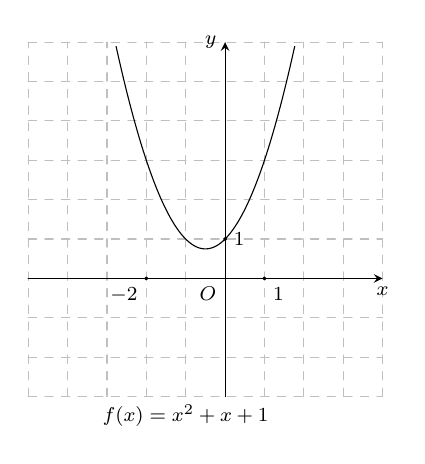
\begin{tikzpicture}[scale=0.5,>=stealth, font=\footnotesize, line join=round, line cap=round]
			\def\a{1} \def\b{1} \def\c{1} % Hệ số
			\def\xmin{-5} \def\xmax{4}
			\def\ymin{-3} \def\ymax{6} 
			\draw[color=gray!50,dashed] (\xmin,\ymin) grid (\xmax,\ymax); 
			\draw[->] (\xmin,0)--(\xmax,0) node [below]{$x$};
			\draw[->] (0,\ymin)--(0,\ymax) node [left]{$y$};
			\node at (0,0) [below left]{$O$};
			\clip (\xmin+0.1,\ymin-1) rectangle (\xmax-0.5,\ymax-0.1);
			\draw[smooth,samples=300] plot(\x,{\a*(\x)^2+\b*(\x)+\c});
			\draw[fill=black]
			(-2,0)node[below left]{$-2$}circle(1pt)
			(1,0)node[below right]{$1$}circle(1pt)
			(0,1)node[right]{$1$}circle(1pt)
			(-1,-3)node[below]{$f(x)=x^2+x+1$};
		\end{tikzpicture}
		\item \newline
		\begin{tikzpicture}[scale=0.5,>=stealth, font=\footnotesize, line join=round, line cap=round]
			\def\a{-9} \def\b{-12} \def\c{-4} % Hệ số
			\def\xmin{-5} \def\xmax{4}
			\def\ymin{-6} \def\ymax{3} 
			\draw[color=gray!50,dashed] (\xmin,\ymin) grid (\xmax,\ymax); 
			\draw[->] (\xmin,0)--(\xmax,0) node [below]{$x$};
			\draw[->] (0,\ymin)--(0,\ymax) node [left]{$y$};
			\node at (0,0) [below right]{$O$};
			\clip (\xmin+0.1,\ymin-1) rectangle (\xmax-0.5,\ymax-0.1);
			\draw[smooth,samples=300,domain=-1.48:0.16] plot(\x,{\a*(\x)^2+\b*(\x)+\c});
			\draw[fill=black]
			(-0.66666,0)node[above]{$-\dfrac{2}{3}$}circle(1pt)
			(0,-4)node[right]{$1$}circle(1pt)
			(-1,-6)node[below]{$f(x)=-9x^2-12x-4$};
		\end{tikzpicture}
		\item \newline
		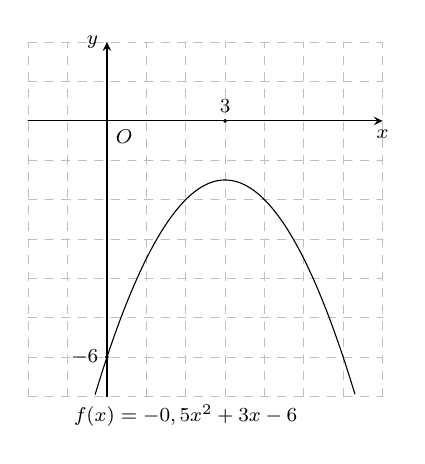
\begin{tikzpicture}[scale=0.5,>=stealth, font=\footnotesize, line join=round, line cap=round]
			\def\a{-0.5} \def\b{3} \def\c{-6} % Hệ số
			\def\xmin{-2} \def\xmax{7}
			\def\ymin{-7} \def\ymax{2} 
			\draw[color=gray!50,dashed] (\xmin,\ymin) grid (\xmax,\ymax); 
			\draw[->] (\xmin,0)--(\xmax,0) node [below]{$x$};
			\draw[->] (0,\ymin)--(0,\ymax) node [left]{$y$};
			\node at (0,0) [below right]{$O$};
			\clip (\xmin+0.1,\ymin-1) rectangle (\xmax-0.5,\ymax-0.1);
			\draw[smooth,samples=300,domain=-0.3:6.3] plot(\x,{\a*(\x)^2+\b*(\x)+\c});
			\draw[fill=black]
			(3,0)node[above]{$3$}circle(1pt)
			(0,-6)node[left]{$-6$}circle(1pt)
			(2,-7)node[below]{$f(x)=-0,5x^2+3x-6$};
		\end{tikzpicture}
		\item \newline
		\begin{tikzpicture}[scale=0.5,>=stealth, font=\footnotesize, line join=round, line cap=round]
			\def\a{-1} \def\b{-0.5} \def\c{3} % Hệ số
			\def\xmin{-5} \def\xmax{4}
			\def\ymin{-4} \def\ymax{5} 
			\draw[color=gray!50,dashed] (\xmin,\ymin) grid (\xmax,\ymax); 
			\draw[->] (\xmin,0)--(\xmax,0) node [below]{$x$};
			\draw[->] (0,\ymin)--(0,\ymax) node [left]{$y$};
			\node at (0,0) [above left]{$O$};
			\clip (\xmin+0.1,\ymin-1) rectangle (\xmax-0.5,\ymax-0.1);
			\draw[smooth,samples=300,domain=-2.9:2.4] plot(\x,{\a*(\x)^2+\b*(\x)+\c});
			\draw[fill=black]
			(-2,0)node[below right]{$-2$}circle(1pt)
			(1.5,0)node[below left]{$\dfrac{3}{2}$}circle(1pt)
			(0,3)node[above right]{$3$}circle(1pt)
			(-1,-4)node[below]{$f(x)=-x^2-0,5x+3$};
		\end{tikzpicture}
		\item \newline
		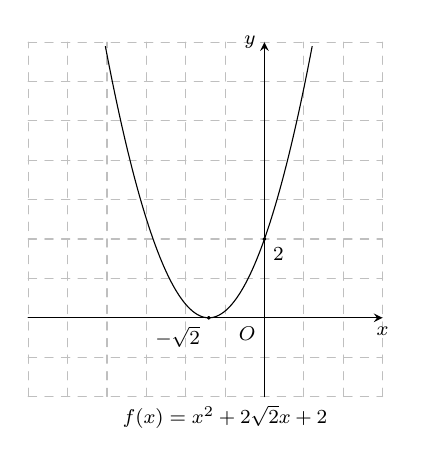
\begin{tikzpicture}[scale=0.5,>=stealth, font=\footnotesize, line join=round, line cap=round]
			\def\a{1} \def\b{2.828427125} \def\c{2} % Hệ số
			\def\xmin{-6} \def\xmax{3}
			\def\ymin{-2} \def\ymax{7} 
			\draw[color=gray!50,dashed] (\xmin,\ymin) grid (\xmax,\ymax); 
			\draw[->] (\xmin,0)--(\xmax,0) node [below]{$x$};
			\draw[->] (0,\ymin)--(0,\ymax) node [left]{$y$};
			\node at (0,0) [below left]{$O$};
			\clip (\xmin+0.1,\ymin-1) rectangle (\xmax-0.5,\ymax-0.1);
			\draw[smooth,samples=300] plot(\x,{\a*(\x)^2+\b*(\x)+\c});
			\draw[fill=black]
			(-1.414213562,0)node[below left]{$-\sqrt{2}$}circle(1pt)
			(0,2)node[below right]{$2$}circle(1pt)
			(-1,-2)node[below]{$f(x)=x^2+2\sqrt{2}x+2$};
		\end{tikzpicture}
	\end{listEX}
	\loigiai{
		\begin{listEX}
			\item Bảng xét dấu
			\begin{center}
				
\begin{tikzpicture}
					\tkzTabInit[,nocadre=false,lgt=2,espcl=2,deltacl=0.5]{$x$/1 ,$f(x)$/1}
					{$-\infty$ , $-2$ , $\dfrac{1}{2}$, $+\infty$}
					\tkzTabLine{,+,0,-,0,+,}
				\end{tikzpicture}
			\end{center}
			\item Bảng xét dấu
			\begin{center}
				
\begin{tikzpicture}
					\tkzTabInit[,nocadre=false,lgt=2,espcl=4,deltacl=0.5]{$x$/1 ,$f(x)$/1}
					{$-\infty$ , $+\infty$}
					\tkzTabLine{,+,}
				\end{tikzpicture}
			\end{center}
			\item Bảng xét dấu
			\begin{center}
				
\begin{tikzpicture}
					\tkzTabInit[,nocadre=false,lgt=2,espcl=2,deltacl=0.5]{$x$/1 ,$f(x)$/1}
					{$-\infty$ , $-\dfrac{2}{3}$, $+\infty$}
					\tkzTabLine{,-,0,-,}
				\end{tikzpicture}
			\end{center}
			\item Bảng xét dấu
			\begin{center}
				
\begin{tikzpicture}
					\tkzTabInit[,nocadre=false,lgt=2,espcl=4,deltacl=0.5]{$x$/1 ,$f(x)$/1}
					{$-\infty$ , $+\infty$}
					\tkzTabLine{,-,}
				\end{tikzpicture}
			\end{center}
			\item Bảng xét dấu
			\begin{center}
				
\begin{tikzpicture}
					\tkzTabInit[,nocadre=false,lgt=2,espcl=2,deltacl=0.5]{$x$/1 ,$f(x)$/1}
					{$-\infty$ , $-2$ , $\dfrac{3}{2}$, $+\infty$}
					\tkzTabLine{,-,0,+,0,-,}
				\end{tikzpicture}
			\end{center}
			\item Bảng xét dấu
			\begin{center}
				
\begin{tikzpicture}
					\tkzTabInit[lgt=2,espcl=2,deltacl=0.5,,nocadre=false]{$x$/1 ,$f(x)$/1}
					{$-\infty$ , $-\sqrt{2}$, $+\infty$}
					\tkzTabLine{,+,0,+,}
				\end{tikzpicture}
			\end{center}
		\end{listEX}
	}
\end{vd}

\begin{vd}%[0D7V1-2]%[Dự án đề cương 3 khối NH24-25 - Đợt 1 - Quan Ón]
	Tìm $m$ để tam thức $f(x) = -x^2 + 2(m-3)x - 5 + m$ nhận giá trị âm với mọi $x \in \mathbb{R}$.
	\loigiai{
		Với mọi $x \in \mathbb{R}$
		\allowdisplaybreaks 
		\begin{eqnarray*}
			f(x)<0 &\Leftrightarrow& \heva{&a<0\\&\Delta <0} \Leftrightarrow \heva{&a=-1<0\\&\Delta =4\cdot (m-3)^2-4\cdot (-1)\cdot \left(-5+m \right)<0}\\
			&\Leftrightarrow& 4m^2-20m+16<0.
		\end{eqnarray*}
		Xét $4m^2-20m+16=0 \Leftrightarrow \hoac{&m=1\\&m=4.}$\\
		Bảng xét dấu
		\begin{center}
			
\begin{tikzpicture}
				\tkzTabInit[deltacl=0.6,espcl=2.5,lgt=4,nocadre=false]
				{$m$/0.8,$4m^2-20m+16$/0.8}
				{$-\infty$,$1$,$4$,$+\infty$}
				\tkzTabLine{,+,0,-,0,+,}
			\end{tikzpicture}
		\end{center}
		Vậy $1<m<4$ thì $f(x)$ âm với mọi $x \in \mathbb{R}$.
	}
\end{vd}

\begin{dang}{Bài toán thực tế}
	Vận dụng kiến thức về dấu của tam thức bậc hai để giải các bài toán thực tế liên quan.
\end{dang}

\begin{vd}%[SGK CD]%[0D7H1-5]%[Dự án đề cương 3 khối NH24-25 - Đợt 1 - Quan Ón]
	Để xây dựng phương án kinh doanh cho một loại sản phẩm, doanh nghiệp tính toán lợi nhuận $y$ (đồng) theo công thức sau $y=-200x^2+92000x-8400000$, trong đó $x$ là số sản phẩm được bán ra. Cho biết doanh nghiệp có lãi khi nào, bị lỗ khi nào.
	\loigiai{
		Xét tam thức bậc hai $f(x)=-200x^2+92000x-8400000$.\\
		$f(x)$ có hai nghiệm là $x_1=\dfrac{-460+\sqrt{43600}}{-2}\approx125{,}6$ và $x_2=\dfrac{-460-\sqrt{43600}}{-2}\approx334{,}4$ và hệ số $a=-200<0$.\\
	    Bảng xét dấu
		\begin{center}
			
\begin{tikzpicture}
				\tkzTabInit[deltacl=0.6,espcl=2.5,lgt=2,nocadre=false]
				{$x$/0.6,$f(x)$/0.6}
				{$-\infty$,$x_1$,$x_2$,$+\infty$}
				\tkzTabLine{,-,0,+,0,-,}
			\end{tikzpicture}
		\end{center}
		Vì $x$ là số nguyên dương nên
		\begin{itemize}
			\item Doanh nghiệp có lãi khi và chỉ khi $f(x)>0$, tức là $126\le x\le334$.
			\item Doanh nghiệp bị lỗ khi và chỉ khi $f(x)<0$, tức là $x\le125$ hoặc $x\ge335$.
		\end{itemize}
		Vậy doanh nghiệp có lãi khi bán từ $126$ đến $334$ sản phẩm, doanh nghiệp bị lỗ khi bán tối đa $125$ sản phẩm hoặc bán tối thiểu $335$ sản phẩm.
	}
\end{vd}

\subsection{Bài tập rèn luyện}
\ind{PHẦN I.} \inden{Câu trắc nghiệm nhiều phương án lựa chọn. Mỗi câu hỏi học sinh chỉ chọn một phương án.}\\
\setcounter{ex}{0}
\Opensolutionfile{ans}[ans/0D7-Bai1-TN]%--Đặt tên 0D7-Bai1-Dang1-TN

\begin{ex}%[0D7N1-1]%[Dự án đề cương 3 khối NH24-25 - Đợt 1 - Quan Ón]
	Biểu thức nào sau đây là tam thức bậc hai?
	\choice
	{$f(x)=-2x+1$}
	{$f(x)=x^3-3x+5$}
	{\True $f(x)=2x^2-5x+2$}
	{$f(x)=-4x^4+x-3$}
	\loigiai{
		Theo định nghĩa thì $f(x)=2x^2-5x+2$ là tam thức bậc hai.
	}
\end{ex}

\begin{ex}%[0D7N1-1]%[Dự án đề cương 3 khối NH24-25 - Đợt 1 - Quan Ón]
	\textit{(Trích đề thi GHKII - Trường THPT Chuyên Lương Thế Vinh - Đồng Nai - Năm học 2024-2025)}\\
	Đa thức nào sau đây là tam thức bậc hai?
	\choice
	{ $f(x) = 2x - 4$}
	{\True $f(x) = 3x^2 + 2x - 5$}
	{ $f(x) = 3x^3 + 2x - 1$}
	{ $f(x) = x^4 - x^2 + 1$}
	\loigiai{
		Tam thức bậc hai có dạng $f(x)=ax^2+bx+c$, ($a \ne 0$) nên $f(x) = 3x^2 + 2x - 5$ là tam thức bậc hai.
	}
\end{ex}

\begin{ex}%[0D7H1-1]%[Dự án đề cương 3 khối NH24-25 - Đợt 1 - Quan Ón]
	Tìm tất cả giá trị của $m$ để biểu thức $f(x)=(m-3)x^2+(2-m)x+1$ là tam thức bậc hai.
	\choice
	{$m=3$}
	{\True $m \neq 3$}
	{$m<3$}
	{$m>3$}
	\loigiai{
		$f(x)=(m-3)x^2+(2-m)x+1$ là tam thức bậc hai khi $m-3\neq 0\Leftrightarrow m\neq 3$.
	}
\end{ex}

\begin{ex}%[0D7H1-1]%[Dự án đề cương 3 khối NH24-25 - Đợt 1 - Quan Ón]
	(\textit{Trích đề thi GHKII - Trường THPT Phan Bội Châu - Bình Thuận - Năm học 2024-2025})\\
	Tất cả các giá trị của $m$ để đa thức $f(x)=\left(m^2-4\right)x^2-3mx+m+1$ là một tam thức bậc hai là
	\choice
	{\True $\left\{\begin{aligned}
			& m\ne 2\\ 
			& m\ne-2\\ 
		\end{aligned}\right.$}
	{$\left[\begin{aligned}
			& m=2\\ 
			& m=-2\\ 
		\end{aligned}\right.$}
	{$ m\ne 2$}
	{$ m\ne-2$}
	\loigiai{
		$f(x)=\left(m^2-4\right)x^2-3mx+m+1$ là một tam thức bậc hai khi và chỉ khi $$m^2-4\ne 0\Leftrightarrow \heva{& m\ne 2 \\ & m\ne -2.}$$
	}
\end{ex}

\begin{ex}%[0D7H1-2]%[Dự án đề cương 3 khối NH24-25 - Đợt 1 - Quan Ón]
	(\textit{Trích đề thi GHKII - Trường THPT Phan Đình Phùng - Hà Nội - Năm học 2024-2025})\\
	Bảng xét dấu nào dưới đây là của tam thức $f(x)=-x^2+4x-4$?
	\choice
	{
\begin{tikzpicture}
			\tkzTabInit[nocadre=false,lgt=1.5,espcl=3,deltacl=0.5]{$x$/1 ,$f(x)$/1}
			{$-\infty$ ,  $2$ , $+\infty$}
			\tkzTabLine{ , + , $0$ , - }
	\end{tikzpicture}}
	{
\begin{tikzpicture}
			\tkzTabInit[nocadre=false,lgt=1.5,espcl=3,deltacl=0.5]{$x$/1 ,$f(x)$/1}
			{$-\infty$ ,  $2$ , $+\infty$}
			\tkzTabLine{ , + , $0$ , + }
	\end{tikzpicture}}
	{
\begin{tikzpicture}
			\tkzTabInit[nocadre=false,lgt=1.5,espcl=3,deltacl=0.5]{$x$/1 ,$f(x)$/1}
			{$-\infty$ ,  $2$ , $+\infty$}
			\tkzTabLine{ , - , $0$ , + }
	\end{tikzpicture}}
	{\True 
\begin{tikzpicture}
			\tkzTabInit[nocadre=false,lgt=1.5,espcl=3,deltacl=0.5]{$x$/1 ,$f(x)$/1}
			{$-\infty$ ,  $2$ , $+\infty$}
			\tkzTabLine{ , - , $0$ , - }
	\end{tikzpicture}}
	\loigiai{Ta có $\Delta ' =0$, phương trình $f(x)=0$ có nghiệm $x=2$ và hệ số $a=-1<0$ nên $f(x)$ có bảng xét dấu là
		\begin{center}
			
\begin{tikzpicture}
				\tkzTabInit[nocadre=false,lgt=1.5,espcl=3,deltacl=0.5]{$x$/1 ,$f(x)$/1}
				{$-\infty$ ,  $2$ , $+\infty$}
				\tkzTabLine{ , - , $0$ , - }
			\end{tikzpicture}
	\end{center}}
\end{ex}

\begin{ex}%[0D7H1-2]%[Dự án đề cương 3 khối NH24-25 - Đợt 1 - Quan Ón]
	Bảng xét dấu nào sau đây là bảng xét dấu của tam thức $f(x)=-x^2-x+6$?
	\choice
	{
\begin{tikzpicture}
			\tkzTabInit[nocadre=false, lgt=1.5, espcl=1.5]
			{$x$ /0.6,$f(x)$ /0.6}
			{$-\infty$,$-2$,$3$, $+\infty$}
			\tkzTabLine{,-,0,+,0,-}
		\end{tikzpicture}
	}
	{
\begin{tikzpicture}
			\tkzTabInit[nocadre=false, lgt=1.5, espcl=1.5]
			{$x$ /0.6,$f(x)$ /0.6}
			{$-\infty$,$-2$,$3$, $+\infty$}
			\tkzTabLine{,+,0,-,0,+}
		\end{tikzpicture}
	}
	{\True 
\begin{tikzpicture}
			\tkzTabInit[nocadre=false, lgt=1.5, espcl=1.5]
			{$x$ /0.6,$f(x)$ /0.6}
			{$-\infty$,$-3$,$2$, $+\infty$}
			\tkzTabLine{,-,0,+,0,-}
		\end{tikzpicture}
	}
	{
\begin{tikzpicture}
			\tkzTabInit[nocadre=false, lgt=1.5, espcl=1.5]
			{$x$ /0.6,$f(x)$ /0.6}
			{$-\infty$,$-3$,$2$, $+\infty$}
			\tkzTabLine{,+,0,-,0,+}
		\end{tikzpicture}
	}
	\loigiai{
		Tam thức $f(x)=-x^2-x-6$ có $\Delta =25>0$, hai nghiệm $x_1=-3$, $x_2=2$ và hệ số $a=-1<0$.\\
		Suy ra bảng xét dấu của $f(x)$ như sau
		\begin{center}
			
\begin{tikzpicture}
				\tkzTabInit[nocadre=false, lgt=1.5, espcl=1.5]
				{$x$ /0.6,$f(x)$ /0.6}
				{$-\infty$,$-3$,$2$, $+\infty$}
				\tkzTabLine{,-,0,+,0,-}
			\end{tikzpicture}
		\end{center}
	}
\end{ex}

\begin{ex}%[0D7H1-2]%[Dự án đề cương 3 khối NH24-25 - Đợt 1 - Quan Ón]
	(\textit{Trích đề thi GHKII - Trường THPT Nguyễn Thị Minh Khai - Hà Nội - Năm học 2024-2025})\\
	Bảng xét dấu nào sau đây là bảng xét dấu của tam thức $f(x)=-x^2+6x-9$?
	\choice
	{
\begin{tikzpicture}
			\tkzTabInit[nocadre=false,lgt=2,espcl=2,deltacl=0.5]
			{$x$/1 , $f(x)$/1}
			{$-\infty$,$3$,$+\infty$}
			\tkzTabLine{,+,z,-}
	\end{tikzpicture}}
	{	
\begin{tikzpicture}
			\tkzTabInit[nocadre=false,lgt=2,espcl=2,deltacl=0.5]
			{$x$/1 , $f(x)$/1}
			{$-\infty$,$3$,$+\infty$}
			\tkzTabLine{,-,z,+}
	\end{tikzpicture}}
	{
\begin{tikzpicture}
			\tkzTabInit[nocadre=false,lgt=2,espcl=2,deltacl=0.5]
			{$x$/1 , $f(x)$/1}
			{$-\infty$,$3$,$+\infty$}
			\tkzTabLine{,+,z,+}
	\end{tikzpicture}}
	{\True 
\begin{tikzpicture}
			\tkzTabInit[nocadre=false,lgt=2,espcl=2,deltacl=0.5]
			{$x$/1 , $f(x)$/1}
			{$-\infty$,$3$,$+\infty$}
			\tkzTabLine{,-,z,-}
	\end{tikzpicture}}
	\loigiai{Ta có $f(x)=0\Leftrightarrow -x^2+6x-9=0\Leftrightarrow x=3$.\\
		Bảng xét dấu 
		\begin{center}
			
\begin{tikzpicture}
				\tkzTabInit[nocadre=false,lgt=2,espcl=2,deltacl=0.5]
				{$x$/1 , $f(x)$/1}
				{$-\infty$,$3$,$+\infty$}
				\tkzTabLine{,-,z,-}
			\end{tikzpicture}
		\end{center}
	}
\end{ex}

\begin{ex}%[0D7H1-2]%[Dự án đề cương 3 khối NH24-25 - Đợt 1 - Quan Ón]
	Tam thức $f(x)=x^2-2x-3$ nhận giá trị dương khi và chỉ khi
	\choice
	{$x\in (-\infty;-3)\cup (-1;+\infty)$}
	{\True $x\in (-\infty;-1)\cup (3;+\infty)$}
	{$x\in (-1;3)$}
	{$x\in (-3;1)$}
	\loigiai{
		Tam thức $f(x)=x^2-2x-3$ có $\Delta=16$, hai nghiệm $x_1=-1$, $x_2=3$ và hệ số $a=1>0$.\\
		Bảng xét dấu của $f(x)$ như sau
		\begin{center}
			
\begin{tikzpicture}
				\tkzTabInit[nocadre=false, lgt=1.5, espcl=1.5]
				{$x$ /0.6,$f(x)$ /0.6}
				{$-\infty$,$-1$,$3$, $+\infty$}
				\tkzTabLine{,+,0,-,0,+}
			\end{tikzpicture}
		\end{center}
		Do đó $f(x)>0\Leftrightarrow x\in (-\infty;-1)\cup (3;+\infty)$.	
	}
\end{ex}

\begin{ex}%[0D7H1-2]%[Dự án đề cương 3 khối NH24-25 - Đợt 1 - Quan Ón]
	Tam thức $f(x)=x^2-12x-13$ nhận giá trị âm khi và chỉ khi
	\choice
	{$x<-13$ hoặc $x>1$}
	{$x<-1$ hoặc $x>13$}
	{$-13<x<1$}
	{\True $-1<x<13$}
	\loigiai{
		Tam thức $f(x)=x^2-12x-13$ có $\Delta =196>0$, hai nghiệm $x_1=-1$, $x_2=13$ và hệ số $a=1>0$.\\
		Bảng xét dấu của $f(x)$ như sau
		\begin{center}
			
\begin{tikzpicture}
				\tkzTabInit[nocadre=false, lgt=1.5, espcl=1.5]
				{$x$ /0.6,$f(x)$ /0.6}
				{$-\infty$,$-1$,$13$, $+\infty$}
				\tkzTabLine{,+,0,-,0,+}
			\end{tikzpicture}
		\end{center}
		Do đó $f(x)<0$ khi $-1<x<13$.
	}
\end{ex}

\begin{ex}%[0D7H1-2]%[Dự án đề cương 3 khối NH24-25 - Đợt 1 - Quan Ón]
	Tam thức bậc hai $f(x)=-x^2+5x-6$ nhận giá trị dương khi và chỉ khi
	\choice
	{$x\in\left(-\infty;2\right)$}
	{$x\in\left(3;+\infty\right)$}
	{$x\in\left(2;+\infty\right)$}
	{\True $x\in\left(2;3\right)$}
	\loigiai
	{Do phương trình $-x^2+5x-6=0$ có hai nghiệm $x=2$, $x=3$ và $a=-1<0$, ta có bảng xét dấu
		\begin{center}
			
\begin{tikzpicture}
				\tkzTabInit[nocadre=false,lgt=1,espcl=3]
				{$x$ /1,$f(x)$/1}{$-\infty$,$2$,$3$,$+\infty$}
				\tkzTabLine{,-,$0$,+,$0$,-,}
			\end{tikzpicture}
		\end{center}
		Từ bảng xét dấu, suy ra tam thức bậc hai $f(x)=-x^2+5x-6$ nhận giá trị dương với $x\in\left(2;3\right)$.}
\end{ex}

\begin{ex}%[0D7H1-2]%[Dự án đề cương 3 khối NH24-25 - Đợt 1 - Quan Ón]
	Tam thức bậc hai $f(x)=x^2+(\sqrt{5}-1)x-\sqrt{5}$ nhận giá trị dương khi và chỉ khi
	\choice
	{$x\in\left(-\sqrt{5};1\right)$}
	{$x\in\left(-\sqrt{5};+\infty\right)$}
	{\True $x\in\left(-\infty;-\sqrt{5}\right)\cup\left(1;+\infty\right)$}
	{$x\in\left(-\infty;1\right)$}
	\loigiai
	{Do phương trình $x^2+(\sqrt{5}-1)x-\sqrt{5}=0$ có hai nghiệm $x=-\sqrt{5}$, $x=1$ và $a=1>0$, ta có bảng xét dấu
		\begin{center}
			\begin{tikzpicture}
				\tkzTabInit[nocadre=false,lgt=1,espcl=3]
				{$x$ /1,$f(x)$/1}{$-\infty$,$-\sqrt{5}$,$1$,$+\infty$}
				\tkzTabLine{,+,$0$,-,$0$,+,}
			\end{tikzpicture}
		\end{center}
		Từ bảng xét dấu, suy ra tam thức bậc hai $f(x)=-x^2+5x-6$ nhận giá trị dương khi và chỉ khi $x\in\left(-\infty;-\sqrt{5}\right)\cup\left(1;+\infty\right)$.}
\end{ex}

\begin{ex}%[0D7H1-2]%[Dự án đề cương 3 khối NH24-25 - Đợt 1 - Quan Ón]
	Cho $f(x)=-x^2+3x-2$ nhận giá trị \textbf{không âm} khi và chỉ khi
	\choice
	{$x\in\left(-\infty;1\right)\cup\left(2;+\infty\right)$}
	{\True $x\in\left[1;2\right]$}
	{$x\in\left(-\infty;1\right]\cup\left[2;+\infty\right)$}
	{$x\in\left(1;2\right)$}
	\loigiai
	{Do phương trình $-x^2+3x-2=0$ có hai nghiệm $x=1$, $x=2$ và $a=-1<0$, ta có bảng xét dấu
		\begin{center}
			\begin{tikzpicture}
				\tkzTabInit[nocadre=false,lgt=1,espcl=3]
				{$x$ /1,$f(x)$/1}{$-\infty$,$1$,$2$,$+\infty$}
				\tkzTabLine{,-,$0$,+,$0$,-,}
			\end{tikzpicture}
		\end{center}
		Từ bảng xét dấu, suy ra tam thức bậc hai $f(x)=-x^2+5x-6$ nhận giá trị không âm khi và chỉ khi $x\in\left[1;2\right]$.}
\end{ex}

\begin{ex}%[0D7H1-2]%[Dự án đề cương 3 khối NH24-25 - Đợt 1 - Quan Ón]
	Cho $f(x)=x^2-4x+3$. Trong các mệnh đề sau, mệnh đề đúng là
	\choice
	{$f(x)<0$ khi và chỉ khi $x\in\left(-\infty;1\right]\cup\left[3;+\infty\right)$}
	{\True $f(x)\leq0$ khi và chỉ khi $x\in\left[1;3\right]$}
	{$f(x)\geq0$ khi và chỉ khi $x\in\left(-\infty;1\right)\cup\left(3;+\infty\right)$}
	{$f(x)>0$ khi và chỉ khi $x\in\left[1;3\right]$}
	\loigiai
	{Do phương trình $x^2-4x+3=0$ có hai nghiệm $x=1$, $x=3$ và $a=1>0$, ta có bảng xét dấu
		\begin{center}
			\begin{tikzpicture}
				\tkzTabInit[nocadre=false,lgt=1,espcl=3]
				{$x$ /1,$f(x)$/1}{$-\infty$,$1$,$3$,$+\infty$}
				\tkzTabLine{,+,$0$,-,$0$,+,}
			\end{tikzpicture}
		\end{center}
		Từ bảng xét dấu, suy ra $f(x)\leq0$ khi $x\in\left[1;3\right]$.}
\end{ex}

\begin{ex}%[0D7H1-2]%[Dự án đề cương 3 khối NH24-25 - Đợt 1 - Quan Ón]
	Dấu của tam thức bậc hai $f(x)=-x^2+5x-6$ được xác định như sau
	\choice
	{$f(x)<0$ với $2<x<3$ và $f(x)>0$ với $x<2$ hoặc $x>3$}
	{$f(x)<0$ với $-3<x<-2$ và $f(x)>0$ với $x<-3$ hoặc $x>-2$}
	{\True $f(x)>0$ với $2<x<3$ và $f(x)<0$ với $x<2$ hoặc $x>3$}
	{$f(x)>0$ với $-3<x<-2$ và $f(x)<0$ với $x<-3$ hoặc $x>-2$}
	\loigiai
	{Do phương trình $-x^2+5x-6=0$ có hai nghiệm $x=2$, $x=3$ và $a=-1<0$, ta có bảng xét dấu
		\begin{center}
			\begin{tikzpicture}
				\tkzTabInit[nocadre=false,lgt=1,espcl=3]
				{$x$ /1,$f(x)$/1}{$-\infty$,$2$,$3$,$+\infty$}
				\tkzTabLine{,-,$0$,+,$0$,-,}
			\end{tikzpicture}
		\end{center}
		Từ bảng xét dấu, suy ra $f(x)>0$ với $2<x<3$ và $f(x)<0$ với $x<2$ hoặc $x>3$.}
\end{ex}


\begin{ex}%[0D7H1-2]%[Dự án đề cương 3 khối NH24-25 - Đợt 1 - Quan Ón]
	Tìm tham số $m$ để tam thức $f(x)=3x^2-2mx+1$ dương tại $x=1$.
	\choice
	{\True $m<2$}
	{$m>2$}
	{$m>-2$}
	{$m<4$}
	\loigiai{
		$f(x)=3x^2-2mx+1$ dương tại $x=1\Leftrightarrow f(1)>0\Leftrightarrow 3-2m+1>0\Leftrightarrow m<2$.	
	}
\end{ex}

\begin{ex}%[0D7H1-3]%[Dự án đề cương 3 khối NH24-25 - Đợt 1 - Quan Ón]
	Dựa vào đồ thị của hàm số bậc hai $y=f(x)$ sau, hãy lập bảng xét dấu của tam thức bậc hai tương ứng.
	\begin{center}
		\begin{tikzpicture}[>=stealth,x=1cm,y=1cm,scale=0.6]
			\def\a{1} % Hệ số a phải khác 0
			\def\b{-4}
			\def\c{3}
			\draw[color=gray,dash pattern=on 1pt off 1pt,xstep=1.0cm,ystep=1.0cm] (-2.2,-2.2) grid (5.2,5.2);
			\draw[->] (-2,0) -- (5,0) node[below] {\scriptsize $x$};
			\draw[->] (0,-2) -- (0,5.5) node[left] {\scriptsize $y$};
			\draw (0,0)node[below right]{\scriptsize $O$};
			\draw (1,0)node[below]{\scriptsize $1$};
			\draw (3,0)node[below]{\scriptsize $3$};
			\draw (0,3)node[left]{\scriptsize $3$};
			\draw (0,-1)node[left]{\scriptsize $-1$};
			\pgfmathsetmacro\xdinh{-(\b)/2*(\a)}
			\pgfmathsetmacro\ydinh{(4*(\a)*(\c)-(\b)^2)/(4*(\a))}
			%	\fill[dashed] (\xdinh,\ydinh)circle(2pt) edge (\xdinh,0) edge (0,\ydinh);
			\clip (-5,-5)rectangle(5,5);
			\draw[thick,samples=150,smooth,domain=-5:5] plot(\x,{\a*(\x)^2+(\b)*\x+(\c)});
		\end{tikzpicture}
	\end{center}	
	\choice
	{\True \begin{tikzpicture}[>=stealth]
			\tkzTabInit[nocadre=false,lgt=1,espcl=1.5,deltacl=0.5]{$x$/.7 ,$f(x)$/.7}
			{$-\infty$ , $1$ ,$3$, $+\infty$}
			\tkzTabLine{ ,+ , $0$, - , $0$ , + , }
		\end{tikzpicture}
	}
	{\begin{tikzpicture}[>=stealth]
			\tkzTabInit[nocadre=false,lgt=1,espcl=1.5,deltacl=0.5]{$x$/.7 ,$f(x)$/.7}
			{$-\infty$ , $1$ ,$3$, $+\infty$}
			\tkzTabLine{ ,- , $0$, + , $0$ , - , }
	\end{tikzpicture}}
	{\begin{tikzpicture}[>=stealth]
			\tkzTabInit[nocadre=false,lgt=1,espcl=1.5,deltacl=0.5]{$x$/.7 ,$f(x)$/.7}
			{$-\infty$ , $1$ ,$3$, $+\infty$}
			\tkzTabLine{ ,- , $0$, - , $0$ , - , }
	\end{tikzpicture}}
	{\begin{tikzpicture}[>=stealth]
			\tkzTabInit[nocadre=false,lgt=1,espcl=1.5,deltacl=0.5]{$x$/.7 ,$f(x)$/.7}
			{$-\infty$ , $1$ ,$3$, $+\infty$}
			\tkzTabLine{ ,+ , $0$, + , $0$ , + , }
	\end{tikzpicture}}
	\loigiai
	{
		Dựa vào đồ thị hàm số đã cho ta xác định được $\Delta>0$ và hệ số $a>0$.\\
		Ta có bảng xét dấu như sau
		\begin{center}
			\begin{tikzpicture}
				\tkzTabInit[nocadre=false,lgt=1.5,espcl=2.5,deltacl=.5]{$x$/1 ,$f(x)$/1}
				{$-\infty$ , $1$, $3$, $+\infty$}
				\tkzTabLine{  ,+,$0$, - ,$0$,+ }
			\end{tikzpicture}
		\end{center}			
	}
\end{ex}

\begin{ex}%[0D7H1-3]%[Dự án đề cương 3 khối NH24-25 - Đợt 1 - Quan Ón]
	Dựa vào đồ thị của hàm số bậc hai $y=f(x)$ sau, hãy lập bảng xét dấu của tam thức bậc hai tương ứng.	
	\begin{center}
		\begin{tikzpicture}[>=stealth,x=1cm,y=1cm,scale=0.6]
			\def\a{1} % Hệ số a phải khác 0
			\def\b{12}
			\def\c{36}
			\draw[color=gray,dash pattern=on 1pt off 1pt,xstep=1.0cm,ystep=1.0cm] (-10.2,-2.2) grid (1.2,5.2);
			\draw[->] (-10,0) -- (1,0) node[below] {\scriptsize $x$};
			\draw[->] (0,-2) -- (0,5.5) node[left] {\scriptsize $y$};
			\draw (0,0)node[below right]{\scriptsize $O$};
			\draw (-6,0)node[below]{\scriptsize $-6$};
			\pgfmathsetmacro\xdinh{-(\b)/2*(\a)}
			\pgfmathsetmacro\ydinh{(4*(\a)*(\c)-(\b)^2)/(4*(\a))}
			%	\fill[dashed] (\xdinh,\ydinh)circle(2pt) edge (\xdinh,0) edge (0,\ydinh);
			\clip (-10,-5)rectangle(2,5);
			\draw[thick,samples=150,smooth,domain=-10:2] plot(\x,{\a*(\x)^2+(\b)*\x+(\c)});
		\end{tikzpicture}
	\end{center}	
	\choice
	{\begin{tikzpicture}[>=stealth]
			\tkzTabInit[nocadre=false,lgt=1,espcl=1.7,deltacl=0.5]{$x$/.7 ,$f(x)$/.7}
			{$-\infty$ , $-6$ , $+\infty$}
			\tkzTabLine{ ,-, $0$ , + , }
		\end{tikzpicture}
	}
	{\begin{tikzpicture}[>=stealth]
			\tkzTabInit[nocadre=false,lgt=1,espcl=1.7,deltacl=0.5]{$x$/.7 ,$f(x)$/.7}
			{$-\infty$ , $-6$ , $+\infty$}
			\tkzTabLine{ ,+, $0$ , - , }
	\end{tikzpicture}}
	{\True \begin{tikzpicture}[>=stealth]
			\tkzTabInit[nocadre=false,lgt=1,espcl=1.7,deltacl=0.5]{$x$/.7 ,$f(x)$/.7}
			{$-\infty$ , $-6$ , $+\infty$}
			\tkzTabLine{ ,+, $0$ , + , }
	\end{tikzpicture}}
	{\begin{tikzpicture}[>=stealth]
			\tkzTabInit[nocadre=false,lgt=1,espcl=1.7,deltacl=0.5]{$x$/.7 ,$f(x)$/.7}
			{$-\infty$ , $-6$ , $+\infty$}
			\tkzTabLine{ ,-, $0$ , - , }
	\end{tikzpicture}}
	\loigiai{
		Dựa vào đồ thị hàm số đã cho ta xác định được $\Delta=0$ và hệ số $a>0$.\\
		Ta có bảng xét dấu như sau
		\begin{center}
			\begin{tikzpicture}
				\tkzTabInit[nocadre=false,lgt=1.5,espcl=3.5,deltacl=.5]{$x$/1 ,$f(x)$/1}
				{$-\infty$ ,$-6$ , $+\infty$}
				\tkzTabLine{  ,+,0,+ , }
			\end{tikzpicture}
		\end{center}	
	}
\end{ex}

\begin{ex}%[0D7H1-3]%[Dự án đề cương 3 khối NH24-25 - Đợt 1 - Quan Ón]
	(\textit{Trích đề thi GHKII - Trường THPT Hải Hậu - Nam Định - Năm học 2024-2025})\\
	Bảng xét dấu sau đây là của tam thức bậc hai nào?
	\begin{center}
		\begin{tikzpicture}
			\tkzTabInit[nocadre=false,lgt=2,espcl=2,deltacl=0.5]{$x$/1 ,$f(x)$/1}
			{$-\infty$ , $2$ , $3$ , $+\infty$}
			\tkzTabLine{ , - , 0 , + , 0 , - ,}
		\end{tikzpicture}
	\end{center}
	\choice
	{$f(x)=x^2-5 x-6$}
	{\True $f(x)=-x^2+5 x-6$}
	{$f(x)=x^2+5 x-6$}
	{$f(x)=-x^2-5 x+6$}
	\loigiai{
		Dựa vào bảng biến thiên ta thấy $ f(x)=0 $ có hai nghiệm phân biệt $ x=2 $, $ x=3 $ và hệ số $ a $ mang dấu âm.\\
		Vậy $f(x)=-x^2+5 x-6$.
	}
\end{ex}

\begin{ex}%[0D7H1-2]%[Dự án đề cương 3 khối NH24-25 - Đợt 1 - Quan Ón]
	Cho $f(x)=ax^2+bx+c$ $(a \neq 0)$ có $\Delta=b^2-4ac<0$. Khi đó mệnh đề nào đúng?
	\choice
	{ $f(x)>0, \forall x \in \mathbb{R}$}
	{ $f(x)<0, \forall x \in \mathbb{R}$}
	{\True $f(x)$ không đổi dấu}
	{ Tồn tại $x$ để $f(x)=0$}
	\loigiai{
		Theo định lý về dấu của tam thức bậc hai, ta có $\Delta <0$	thì $f(x)$ luôn cùng dấu với hệ số $a$, do đó $f(x)$ không đổi dấu.
	}
\end{ex}

\begin{ex}%[0D7H1-2]%[Dự án đề cương 3 khối NH24-25 - Đợt 1 - Quan Ón]
	(\textit{Trích đề thi GHKII - Trường THPT Phan Đình Phùng - Hà Nội - Năm học 2024-2025})\\
	Cho tam thức $f(x)=a x^2+b x+c\ (a \neq 0)$ với $\Delta=b^2-4a c$. Ta có $f(x) > 0$ với $\forall x \in \mathbb{R}$ khi và chỉ khi:
	\choice
	{$\heva{&a < 0\\&\Delta > 0}$}
	{$\heva{&a < 0\\&\Delta \geq 0}$}
	{$\heva{&a > 0\\&\Delta > 0}$}
	{\True $\heva{&a > 0\\&\Delta < 0}$}
	\loigiai{
		Ta có $f(x) > 0,\forall x \in \mathbb{R} \Leftrightarrow \heva{&a > 0\\&\Delta < 0.}$
	}
\end{ex}

\begin{ex}%[0D7H1-2]%[Dự án đề cương 3 khối NH24-25 - Đợt 1 - Quan Ón]
	Cho $f(x)=ax^2+bx+c$ $(a \neq 0)$. Điều kiện để $f(x) \geq 0, \forall x \in \mathbb{R}$ là
	\choice
	{\True $\heva{&a>0 \\& \Delta \leq 0}$}
	{ $\heva{&a>0 \\& \Delta \geq 0}$}
	{ $\heva{&a>0 \\& \Delta<0}$}
	{ $\heva{&a<0 \\& \Delta>0}$}
	\loigiai{
		Ta có $f(x) \geq 0, \forall x \in \mathbb{R} \Leftrightarrow \heva{&a>0 \\& \Delta \leq 0.}$
	}
\end{ex}

\begin{ex}%[0D7H1-2]%[Dự án đề cương 3 khối NH24-25 - Đợt 1 - Quan Ón]
	Cho $f(x)=a x^2+bx+c$ $(a \neq 0)$. Điều kiện để $f(x)<0, \forall x \in \mathbb{R}$ là
	\choice
	{ $\heva{&a<0 \\& \Delta \leq 0}$}
	{ $\heva{&a<0 \\& \Delta=0}$}
	{ $\heva{&a>0 \\& \Delta<0}$}
	{\True $\heva{&a<0 \\& \Delta<0}$}
	\loigiai{
		Ta có $f(x)<0, \forall x \in \mathbb{R} \Leftrightarrow \heva{&a<0 \\& \Delta<0.}$
	}
\end{ex}

\begin{ex}%[0D7H1-2]%[Dự án đề cương 3 khối NH24-25 - Đợt 1 - Quan Ón]
	Cho $f(x)=a x^2+bx+c$ $(a \neq 0)$. Điều kiện để $f(x) \leq 0, \forall x \in \mathbb{R}$ là
	\choice
	{\True $\heva{&a<0 \\& \Delta \leq 0}$}
	{ $\heva{&a<0 \\& \Delta \geq 0}$}
	{ $\heva{&a>0 \\& \Delta<0}$}
	{ $\heva{&a<0 \\& \Delta>0}$}
	\loigiai{
		Ta có $f(x) \leq 0, \forall x \in \mathbb{R} \Leftrightarrow \heva{&a<0 \\& \Delta \leq 0.}$
	}
\end{ex}

\begin{ex}%[0D7H1-2]%[Dự án đề cương 3 khối NH24-25 - Đợt 1 - Quan Ón]
	(\textit{Trích đề thi GHKII - Trường THPT Phan Bội Châu - Bình Thuận - Năm học 2024-2025})\\
	Cho tam thức bậc hai $f(x)=ax^2+bx+c$ với $ a<0$ và $\Delta <0$. Khẳng định nào dưới đây đúng?
	\choice
	{\True $ f(x)<0,\forall x\in\mathbb{R}$}
	{$ f(x)>0,\forall x\in\mathbb{R}$}
	{$ f(x)>0,\forall x\in\mathbb{R}\setminus\left\{-\dfrac{b}{2a}\right\}$}
	{$ f(x)\ge 0,\forall x\in\mathbb{R}$}
	\loigiai{
		Ta có $f(x)=ax^2+bx+c<0,\forall x\in\mathbb{R}\Leftrightarrow \heva{& a<0 \\ & \Delta <0.}$}
\end{ex}

\begin{ex}%[0D7H1-3]%[Dự án đề cương 3 khối NH24-25 - Đợt 1 - Quan Ón]
	(\textit{Trích đề thi GHKII - Trường THPT Phạm Văn Đồng - Quảng Ngãi - Năm học 2024-2025})\\
	\immini{Đồ thị của hàm số $f(x)=a{x^2}+bx+c$ như hình vẽ. Tìm mệnh đề đúng?
		\choice
		{$\heva{
				& a>0\\ 
				&\Delta\le 0\\ 
			}$}
		{\True $\heva{
				& a>0\\ 
				&\Delta <0\\ 
			}$}
		{$\heva{
				& a>0\\ 
				&\Delta >0\\ 
			}$}
		{$\heva{
				& a<0\\ 
				&\Delta <0\\ 
			}$}}{\begin{tikzpicture}[line join=round, line cap=round,>=stealth,font=\footnotesize,scale=0.6]
			\tikzset{every node/.style={scale=0.8}}
			\draw[->] (-2.1,0)--(4.1,0) node[below left] {$x$};
			\draw[->] (0,-1.1)--(0,5.1) node[below left] {$y$};
			\draw (0,0) node [below left] {$O$};
			\foreach \x/\nx in {1/1}
			\draw[thin] (\x,1pt)--(\x,-1pt) node [below] {$\nx$};
			\foreach \y/\ny in {2/2}
			\draw[thin] (1pt,\y)--(-1pt,\y) node [left] {$\ny$};
			\begin{scope}
				\clip (-2,-1) rectangle (4,5);
				\draw[samples=200,domain=-1:3,smooth,variable=\x] plot (\x,{1*(\x)^2-2*(\x)+2});
				\draw[samples=200,domain=-1:3,smooth,variable=\x] plot (\x,{1*(\x)^2-2*(\x)+2});
			\end{scope}
	\end{tikzpicture}}
	\loigiai{
		Parabol có bề lõm hướng lên nên $a>0$. Parabol không cắt trục $Ox$ nên phương trình $ a{x^2}+bx+c=0$ vô nghiệm, tức là $\Delta <0$.}
\end{ex}

\begin{ex}%[0D7V1-2]%[Dự án đề cương 3 khối NH24-25 - Đợt 1 - Quan Ón]
	Tam thức $f(x)=x^{2}+2\left(2m+3\right)x+5m+6$ nhận giá trị dương với mọi $x$ khi và chỉ khi
	\choice
	{ $m\leqslant -1$ hoặc $m\geqslant -\dfrac{3}{4}$}
	{ $m<-1$ hoặc $m>-\dfrac{3}{4}$}
	{ $-1\leqslant m\leqslant -\dfrac{3}{4}$}
	{\True $-1<m<-\dfrac{3}{4}$}
	\loigiai{
		Ta có $f(x)>0,\ \forall x\in \mathbb{R}\Leftrightarrow \heva{&a>0 \\& \Delta <0}\Leftrightarrow \heva{&1>0 \text{ (luôn đúng)}\\&4m^2+7m+3<0& }\Leftrightarrow -1<m<-\dfrac{3}{4}$.
	}
\end{ex}

\begin{ex}%[0D7H1-4]%[Dự án đề cương 3 khối NH24-25 - Đợt 1 - Quan Ón]
	(\textit{Trích đề thi GHKII - Trường THPT Phạm Văn Đồng - Quảng Ngãi - Năm học 2024-2025})\\
	Cho biểu thức $ f(x)=x^2\left(x^2-4\right)$ có bảng xét dấu như sau
	\begin{center}
		\begin{tikzpicture}
			\tkzTabInit[nocadre=false,lgt=2,espcl=2,deltacl=0.5]{$x$/1 ,$f(x)$/1}
			{$-\infty$ , $-2$ , $0$ , $2$ , $+\infty$}
			\tkzTabLine{  , ? , 0 , ? , 0 , ? , 0 ,? }
		\end{tikzpicture}
	\end{center}
	Dấu trong các dấu chấm hỏi theo thứ tự từ trái sang phải là
	\choice
	{\True $+,-,-,+$}
	{$+,-,+,-$}
	{$-,+,-,+$}
	{$+,+,-,+$}
	\loigiai{
		Ta có $ f(x)=0\Leftrightarrow\hoac{&x=0\\&
			x=\pm 2.}$\\ 
		Ta có bảng xét dấu $ f(x)=x^2\left(x^2-4\right)$ như sau
		\begin{center}
			\begin{tikzpicture}
				\tkzTabInit[nocadre=false,lgt=2,espcl=2,deltacl=0.5]{$x$/1 ,$f(x)$/1}
				{$-\infty$ , $-2$ , $0$ , $2$ , $+\infty$}
				\tkzTabLine{  , + , 0 , - , 0 , - , 0 ,+ }
			\end{tikzpicture}
	\end{center}}
\end{ex}

\begin{ex}%[0D7H1-2]%[Dự án đề cương 3 khối NH24-25 - Đợt 1 - Quan Ón]
	(\textit{Trích đề thi GHKII - Trường THPT Nguyễn Thị Minh Khai - Hà Nội - Năm học 2024-2025})\\
	Cho $f(x)=ax^2+bx+c$, $(a\neq 0)$ và $\Delta=b^2-4ac$. Cho biết dấu của $\Delta$ khi $f(x)$ luôn cùng dấu với hệ số $a$ với mọi $x\in \mathbb{R}$.
	\choice
	{\True $\Delta<0$}
	{$\Delta=0$}
	{$\Delta>0$}
	{$\Delta\geq 0$}
	\loigiai{Theo định lí dấu của tam thức bậc hai thì $f(x)$ luôn cùng dấu với hệ số $a$ với mọi $x\in \mathbb{R}$ khi $\Delta<0$.}
\end{ex}

\Closesolutionfile{ans}

\ind{PHẦN II.} \inden{Câu trắc nghiệm đúng sai. Trong mỗi ý a), b), c), d) ở mỗi câu, học sinh chọn đúng hoặc sai.}\\
\setcounter{ex}{0}
\Opensolutionfile{ans}[ans/0D7-Bai1-DS]%--Đặt tên 2D1-Bai1-DS

\begin{ex}%[0D7H1-2]%[Dự án đề cương 3 khối NH24-25 - Đợt 1 - Quan Ón]
	(\textit{Trích đề thi GHKII - Trường Chuyên Nguyễn Đình Chiều - Đồng Tháp - Năm học 2024-2025})\\
	Cho tam thức bậc hai $f(x)=x^2+2m x-2m+3$, với $m$ là tham số.
	\choiceTF
	{Với $m=1$, thì $f(x)=x^2+3$}
	{\True $f(1) > 0$, $\forall m \in \mathbb{R}$}
	{\True $f(x) > 0, \forall x \in \mathbb{R} \Leftrightarrow m \in(-3; 1)$}
	{$f(x)$ có hai nghiệm phân biệt khi $-3<m<1$}
	\loigiai{
		\begin{itemchoice}
			\itemch \textbf{Sai.} Với $m=1$ thì $f(x)=x^2+2x+1\neq x^2+3$.
			\itemch \textbf{Đúng.} Ta có $f(1)=4>0$, $\forall m \in \mathbb{R}$.
			\itemch \textbf{Đúng.} Ta có $\Delta = 4m^2+8m-12$.\\
			Để $f(x)>0$, $\forall m \in \mathbb{R}$ thì $\heva{&a>0\\&\Delta < 0} \Leftrightarrow \heva{&4 > 0 \text{ (luôn đúng)}\\&4m^2+8m-12 
			< 0} \Leftrightarrow 4m^2+8m-12 
			< 0$.\\
			Xét tam thức bậc hai $f(m) = 4m^2+8m-12$.\\
			Ta có $f(m) = 0 \Leftrightarrow 4m^2+8m-12 = 0 \Leftrightarrow \hoac{&m=-3\\&m=1.}$\\
			Hệ số $a = 4 > 0$.\\
			Bảng xét dấu
			\begin{center}
				\begin{tikzpicture}
					\tkzTabInit[nocadre=false,lgt=2,espcl=2,deltacl=0.5]{$m$/1 ,$f(m)$/1}
					{$-\infty$, $-3$, $1$, $+\infty$}
					\tkzTabLine{  , + , 0 , - , 0 , + }
				\end{tikzpicture}
			\end{center}
			Dựa vào bảng xét dấu, ta thấy $f(m) < 0$ khi $-3 < m < 1$.\\
			\itemch \textbf{Sai.} Dựa vào bảng xét dấu thì $f(x)$ có hai nghiệm phân biệt khi $\Delta>0$, tức là $m\in \left(-\infty;-3\right)\cup\left(1;+\infty\right)$.
		\end{itemchoice}
	}
\end{ex}

\begin{ex}%[0D7H1-3]%[Dự án đề cương 3 khối NH24-25 - Đợt 1 - Quan Ón]
	(\textit{Trích đề thi GHKII - Trường Ea H'Leo - Đắk Lắk - Năm học 2024-2025})\\
	Đường parabol trong hình dưới là đồ thị của một hàm bậc hai $y=f(x)=ax^2 + bx + c$ $(a \neq 0)$.
	\begin{center}
		\begin{tikzpicture}[line join = round, line cap=round,>=stealth,font=\footnotesize,scale=0.7]
			\path 
			(0,0) coordinate (O) node[below left]{$O$}
			(3.9,0) coordinate (X) node[below]{$x$}
			(0,2) coordinate (Y) node[right]{$y$}
			;
			\draw[->] (-2,0)--(4,0);
			\draw[->] (0,-5)--(0,2.2);
			\draw[smooth] plot[domain=-1.5:3.5] (\x,{(\x)^2-2*\x-3});
			\draw[dashed] (1,0)--(1,-4)--(0,-4);
			\fill (-1,0) circle (1pt) node[below left]{$-1$};
			\fill (1,0) circle (1pt) node[above]{$1$};
			\fill (3,0) circle (1pt) node[below right]{$3$};
			\fill (0,-4) circle (1pt) node[left]{$-4$};
			\fill (0,1) circle (1pt) node[left]{$1$};
		\end{tikzpicture}
	\end{center}
	\choiceTF
	{Hàm số đồng biến trên khoảng $(-4; +\infty)$ và nghịch biến trên khoảng $(-\infty; -4)$}
	{\True Đồ thị hàm số bậc hai đi qua các điểm có toạ độ $(3;0)$, $(-1;0)$ và $(1;-4)$}
	{Xét dấu tam thức được kết quả $f(x)>0$, $\forall x \in (1; +\infty)$ và $f(x)<0$, $\forall x \in (-\infty; 1)$}
	{\True Giá trị biểu thức $a+b=-1$}
	\loigiai{
		\begin{itemchoice}
			\itemch \textbf{Sai.} Vì hàm số đồng biến trên khoảng từ $(1; +\infty)$ và nghịch biến trên khoảng $(-\infty;1)$.
			\itemch \textbf{Đúng.} Dựa vào hình vẽ ta thấy, đồ thị hàm số bậc hai đi qua các điểm có toạ độ $(3;0)$; $(-1;0)$ và $(1;-4)$.
			\itemch \textbf{Sai.} Xét dấu tam thức được kết quả: $f(x)>0$, $\forall x \in (-\infty;-1) \cup (3; +\infty)$ và $f(x)<0$, $\forall x \in (-1; 3)$.
			\itemch \textbf{Đúng.} Vì đồ thị hàm số bậc hai $y=f(x)=ax^2 + bx + c$ đi qua các điểm có toạ độ $(3;0)$; $(-1;0)$ và $(1;-4)$ nên ta có hệ
			\[\heva{&a-b+c=0 \\& 9a +3b+c=0 \\&a+b+c=-4} \Leftrightarrow \heva{&a=1 \\&b=-2 \\&c=-3.}\]
			Vậy $a+b=1+(-2)=-1$.
		\end{itemchoice}
	}
\end{ex}

\begin{ex}%[0D7H1-2]%[Dự án đề cương 3 khối NH24-25 - Đợt 1 - Quan Ón]
	Cho tam thức bậc hai $f(x)=-2x^2+7x-3$.
	\choiceTF
	{\True Tam thức $f(x)$ có hai nghiệm phân biệt $x=\dfrac{1}{2}$ và $x=3$}
	{$f(x)<0$ khi và chỉ khi $\dfrac{1}{2}<x<3$}
	{\True $f(x)\ge 0$ có $3$ nghiệm nguyên}
	{\True $f(x)<0,\forall x\in (-\infty;m+2)$ khi và chỉ khi $m\le-\dfrac{3}{2}$}
	\loigiai{
		Ta có $-2x^2+7x-3=0\Leftrightarrow \hoac{&x=\dfrac{1}{2}\\&x=3.}$\\
		Bảng xét dấu
		\begin{center}
			\begin{tikzpicture}
				\tkzTabInit[nocadre=false, lgt=2, espcl=2.5]
				{$x$ /1,$f(x)$ /1}
				{$-\infty$,$\dfrac{1}{2}$,$3$,$+\infty$}
				\tkzTabLine{,-,$0$,+,$0$,-,}
			\end{tikzpicture}
		\end{center}
		\begin{itemchoice}
			\itemch \textbf{Đúng.}\\
			Ta có $f(x)$ có hai nghiệm phân biệt $x=\dfrac{1}{2}$ và $x=3$.
			\itemch \textbf{Sai.}\\
			Từ bảng xét dấu, ta có $f(x)<0$ khi và chỉ khi $x\in \left(-\infty;\dfrac{1}{2}\right)\cup (3;+\infty)$. 
			\itemch \textbf{Đúng.}\\
			Từ bảng xét dấu, ta có $f(x)\ge 0$ khi và chỉ khi $x\in \left[\dfrac{1}{2};3\right]$.\\
			Do đó bất phương trình $f(x)\ge 0$ có $3$ nghiệm nguyên là $\{1; 2; 3\}$.
			\itemch \textbf{Đúng.}\\
			$f(x)<0\,\forall x\in (-\infty;m+2)$ khi và chỉ khi
			$$m+2\le \dfrac{1}{2}\Leftrightarrow m\le -\dfrac{3}{2}.$$
		\end{itemchoice}
	}
\end{ex}

\begin{ex}%[0D7H1-3]%[Dự án đề cương 3 khối NH24-25 - Đợt 1 - Quan Ón]
	Cho tam thức bậc hai $f(x)$ có đồ thị như hình vẽ sau
	\begin{center}
		\begin{tikzpicture}[line join=round, line cap=round,>=stealth,thick]
			\tikzset{every node/.style={scale=0.9}}
			\draw[->] (-1.1,0)--(4.1,0) node[below left] {$x$};
			\draw[->] (0,-2.1)--(0,3.1) node[below left] {$y$};
			\draw (0,0) node [below left] {$O$};
			\draw[dashed](2,0)--(2,2)--(0,2);
			\fill (2,0)node[below]{$2$} (0,2)node[left]{$2$} (2,2)circle(1.5pt) (1,0)node[below left]{$1$}circle(1.5pt) (3,0)node[below right]{$3$}circle(1.5pt);
			\begin{scope}
				\clip (-1,-2) rectangle (4,3);
				\draw[samples=200,domain=-1.5:4.5,smooth,variable=\x] plot (\x,{-2*(\x)^2+8*(\x)+-6});
			\end{scope}
		\end{tikzpicture}
	\end{center}
	\choiceTF
	{\True Tam thức bậc hai $f(x)$ có $\Delta > 0$}
	{\True Tam thức bậc hai $f(x)$ có hai nghiệm $x=1;x=3$}
	{Tam thức bậc hai $f(x)$ có hệ số $a > 0$}
	{$f(x) < 2$ có tập nghiệm $S=\mathbb{R}$}
	\loigiai{
		\begin{itemchoice}
			\itemch \textbf{Đúng.} Vì đồ thị cắt $Ox$ tại $2$ điểm phân biệt nên tam thức bậc hai $f(x)$ có $\Delta > 0$.			
			\itemch \textbf{Đúng.} Dựa vào đồ thị, ta có $f(x) = 0 \Leftrightarrow \hoac{&x = 1\\&x = 3.}$\\
			Do đó, tam thức bậc hai $f(x)$ có hai nghiệm $x=1$; $x=3$.
			\itemch \textbf{Sai.}\\
			Vì đồ thị hàm số $f(x)$ là parabol quay bề lõm xuống dưới nên hệ số $a<0$.
			\itemch \textbf{Sai.} Thật vậy, ta thấy đường thẳng $y=2$ tiếp xúc với đồ thị của $f(x)$ tại điểm $(2;2)$ và phần đồ thị còn lại của $f(x)$ luôn nằm dưới đường thẳng nên bất phương trình $f(x)<2$ có tập nghiệm là $S=\mathbb{R}\setminus\{2\}$.
		\end{itemchoice}
	}
\end{ex}

\begin{ex}%[0D7H1-3]%[Dự án đề cương 3 khối NH24-25 - Đợt 1 - Quan Ón]
	Cho tam thức bậc hai $y=f(x)=a{x^2}+bx+c$ có đồ thị như hình vẽ bên dưới.
	\begin{center}
		\begin{tikzpicture}[line join=round, line cap=round,>=stealth,thick]
			\tikzset{every node/.style={scale=0.9}}
			\draw[->] (-1.1,0)--(4.1,0) node[below left] {$x$};
			\draw[->] (0,-2.1)--(0,3.1) node[below left] {$y$};
			\draw (0,0) node [below left] {$O$};
			
			\fill (-1,0)node[below]{$-1$} (2,0)node[below]{$2$}    (1,0)node[below left]{$1$}  (3,0)node[below right]{$3$};
			\begin{scope}
				\clip (-1,-2) rectangle (4,3);
				\draw[samples=200,domain=-1.5:4.5,smooth,variable=\x] plot (\x,{1*(\x)^2-2*(\x)});
			\end{scope}
		\end{tikzpicture}
	\end{center}
	\choiceTF
	{\True $f(x)$ có hệ số $a>0$}
	{Tam thức bậc hai $f(x)$ có $\Delta <0$}
	{\True $f(x)$ âm trên khoảng $(0;2)$}
	{\True $f(x)$ dương trên khoảng $(2;+\infty)$}
	\loigiai{
		Từ đồ thị ta có bảng xét dấu của $f(x)$ như sau
		\begin{center}
			\begin{tikzpicture}
				\tkzTabInit[nocadre=false, lgt=2, espcl=2.5]
				{$x$ /1,$f(x)$ /1}
				{$-\infty$,$0$,$2$,$+\infty$}
				\tkzTabLine{,+,$0$,-,$0$,+,}
			\end{tikzpicture}
		\end{center}
		Do đó
		\begin{itemchoice}
			\itemch \textbf{Đúng.}\\
			Từ đồ thị hàm số $y=f(x)$, suy ra $a>0$.			
			\itemch \textbf{Sai.}\\
			Vì đồ thị hàm số $y=f(x)$ cắt trục hoành tại hai điểm nên $f(x)$ có $\Delta>0$.
			\itemch \textbf{Đúng.}\\
			Dựa vào bảng xét dấu, ta thấy $f(x) < 0$ khi $x \in (0;2)$.\\
			Do đó $f(x)$ âm trên khoảng $(0;2)$.
			\itemch \textbf{Đúng.}\\
			Vì $f(x)>0\Leftrightarrow x\in (-\infty;0)\cup (2;+\infty)$.
		\end{itemchoice}	
	}
\end{ex}


\Closesolutionfile{ans}


\ind{PHẦN III.} \inden{Câu trắc nghiệm trả lời ngắn.}\\
\setcounter{ex}{0}
\Opensolutionfile{ans}[ans/0D7-Bai1-TLN]%--Đặt tên 2D1-Bai1-TLN

\begin{ex}%[0D7H1-1]%[Dự án đề cương 3 khối NH24-25 - Đợt 1 - Quan Ón]
	Cho tam thức bậc hai $f(x) = 2x^2 + x - 3$. Tổng các nghiệm của tam thức bằng bao nhiêu?
	\shortans{$-0{,}5$}
	\loigiai{
		Ta có tam thức có hai nghiệm $x_1=1$; $x_2 = \dfrac{-3}{2}$ suy ra $x_1 + x_2 = \dfrac{-1}{2} = -0{,}5$.
	}
\end{ex}


\begin{ex}%[0D7V1-2]%[Dự án đề cương 3 khối NH24-25 - Đợt 1 - Quan Ón]
	Cho tam thức bậc hai $f(x) = 2x^2-3x-15$. Có bao nhiêu giá trị nguyên của $x$ để $f(x) \leq 0$ là
	\shortans{$6$}
	\loigiai{
		Giải bất phương trình $2x^2-3x-15 \le 0$. \\
		Bảng xét dấu
		\begin{center}
			\begin{tikzpicture}
				\tkzTabInit
				[lgt=4,espcl=0.007\linewidth]
				{$x$/1, $2x^2-3x-15$/1}
				{$-\infty$,$\dfrac{3-\sqrt{129}}{4}$, $\dfrac{3+\sqrt{129}}{4}$, $+\infty$}
				\tkzTabLine{,+, $0$, -, $0$, +,}
			\end{tikzpicture}
		\end{center}
		Dựa vào bảng xét dấu ta được $\dfrac{3-\sqrt{129}}{4} \le x\le \dfrac{3+\sqrt{129}}{4}$. \\
		Suy ra $x$ có $6$ giá trị nguyên: $\{-2; -1; 0; 1; 2; 3\}$.
	}
\end{ex}


\begin{ex}%[0D7V1-1]%[Dự án đề cương 3 khối NH24-25 - Đợt 1 - Quan Ón]
	Cho tam thức bậc hai $f(x)=2x^2+9x-5$. Có bao nhiêu giá trị nguyên của tham số $m$ để $f(x)$ luôn âm với mọi $x\in (m;2m-1)$?
	\shortans{$0$}
	\loigiai{
		Ta có $f(x)=2x^2+9x-5=0\Leftrightarrow x=-5$ hoặc $x=\dfrac{1}{2}$.\\
		Bảng xét dấu
		\begin{center}
			\begin{tikzpicture}
				\tkzTabInit[nocadre=false, lgt=2, espcl=2.5]
				{$x$ /1,$f(x)$ /1}
				{$-\infty$,$-5$,$\dfrac{1}{2}$,$+\infty$}
				\tkzTabLine{,+,$0$,-,$0$,+,}
			\end{tikzpicture}
		\end{center}
		Do đó $f(x)$ luôn âm với mọi $x\in (m;2m-1)$ khi và chỉ khi
		$$-5\le m<2m-1\le \dfrac{1}{2}\Leftrightarrow \heva{&m \geq -5\\&m < 2m - 1\\&2m - 1\leq \dfrac{1}{2}} \Leftrightarrow \heva{&m \geq -5\\&m > 1\\&m \leq \dfrac{3}{4}} \Rightarrow m \in \varnothing.$$
		Vậy không có giá trị nguyên của $m$ thỏa mãn.
	}
\end{ex}


\begin{ex}%[0D7V1-2]%[Dự án đề cương 3 khối NH24-25 - Đợt 1 - Quan Ón]
	Cho tam thức bậc hai $f(x) = x^2 - 4x + 3$. Biết rằng $f(x)$ luôn âm với mọi $x \in (a;b)$. Khi đó $b-a$ bằng bao nhiêu?
	\shortans{$2$}
	\loigiai{
		Bảng xét dấu
		\begin{center}
			\begin{tikzpicture}
				\tkzTabInit
				[lgt=4,espcl=0.007\linewidth]
				{$x$/1, $x^2-4x+3$/1}
				{$-\infty$,$1$, $3$, $+\infty$}
				\tkzTabLine{,+, $0$, -, $0$, +,}
			\end{tikzpicture}
		\end{center}
		Dựa vào bảng xét dấu, ta thấy $f(x) < 0$ khi $1 < x < 3$. \\
		Do đó $a = 1$ và $b = 3 \Rightarrow b - a = 3 - 1 = 2$.
	}
\end{ex}

\begin{ex}%[0D7V1-2]%[Dự án đề cương 3 khối NH24-25 - Đợt 1 - Quan Ón]
	Cho tam thức bậc hai $f(x)=x^2+9x+8$. Tập hợp các giá trị của $m$ để $f(x)$ luôn âm với mọi $x\in (3m;2m+3)$ là đoạn $[a;b]$, tính $a\cdot b$ (\textit{kết quả lấy gần đúng đến hàng phần trăm}).
	\shortans{$5{,}33$}
	\loigiai{
		Ta có $f(x)=x^2+9x+8=0\Leftrightarrow x=-8$ hoặc $x=-1$.\\
		Bảng xét dấu
		\begin{center}
			\begin{tikzpicture}
				\tkzTabInit[nocadre=false, lgt=2, espcl=2.5]
				{$x$ /1,$f(x)$ /1}
				{$-\infty$,$-8$,$-1$,$+\infty$}
				\tkzTabLine{,+,$0$,-,$0$,+,}
			\end{tikzpicture}
		\end{center}
		Do đó $f(x)$ luôn âm với mọi $x\in (3m;2m+3)$ khi và chỉ khi
		$$-8\le 3m<2m+3\le -1\Leftrightarrow -\dfrac{8}{3}\le m\le-2.$$
		Từ đó ta có $a=-\dfrac{8}{3}$ và $b=-2$. Do đó $a\cdot b=\left(-\dfrac{8}{3}\right)\cdot (-2)\approx 5{,}33$.
	}
\end{ex}

\Closesolutionfile{ans}


\ind{PHẦN IV.} \inden{Tự luận.}\\
\setcounter{ex}{0}

\begin{ex}%[0D7N1-1]%[Dự án đề cương 3 khối NH24-25 - Đợt 1 - Quan Ón]
	Hãy cho biết biểu thức nào sau đây là tam thức bậc hai?
	\begin{multicols}{3}
		\begin{enumerate}
			\item $f(x) = 3x+2\sqrt{x}+1$.
			\item $f(x) = -5x^4+3x^2+4$.
			\item $f(x) = -\dfrac{2}{3}x^2+7x-4$.
			\item $f(x) = \left(\dfrac{1}{x}\right)^2+2\dfrac{1}{x}+3$.
			\item $f(x) = x^2 - 4x + 1$.
			\item $f(x) = 2x^2 + 1$.
		\end{enumerate}
	\end{multicols}
	\loigiai{
		\begin{enumerate}
			\item Biểu thức $f(x) = 3x+2\sqrt{x}+1$ không là tam thức bậc hai.
			\item Biểu thức $f(x) = -5x^4+3x^2+4$ không là tam thức bậc hai.
			\item Biểu thức $f(x) = -\dfrac{2}{3}x^2+7x-4$ là tam thức bậc hai.
			\item Biểu thức $f(x) = \left(\dfrac{1}{x}\right)^2+2\dfrac{1}{x}+3$ không là tam thức bậc hai.
			\item Biểu thức $f(x) = x^2 - 4x + 1$ là tam thức bậc hai.
			\item Biểu thức $f(x) = 2x^2 + 1$ là tam thức bậc hai.
		\end{enumerate}
	}
\end{ex}

\begin{ex}%[0D7H1-1]%[Dự án đề cương 3 khối NH24-25 - Đợt 1 - Quan Ón]
	Tìm các giá trị của tham số $m$ để
	\begin{enumerate}
		\item $f(x)=(2m-8)x^2+2mx+1$ là một tam thức bậc hai.
		\item $f(x)=(2m+3)x^2+3x-4m^2$ là một tam thức bậc hai có $x=3$ là một nghiệm.
		\item $f(x)=2x^2+mx-3$ dương tại $x=2$.
	\end{enumerate}
	\loigiai{
		\begin{enumerate}
			\item $f(x)$ là tam thức bậc hai khi và chỉ khi $2m-8 \ne 0$, hay $m \ne 4$.
			\item $f(x)$ là tam thức bậc hai khi và chỉ khi $2m+3 \ne 0$, tức là $m \ne -\dfrac{3}{2}$.\\
			$f(x)$ có $x=3$ là nghiệm khi
			$$ f(3)=9(2m+3)+9-4m^2=0\Leftrightarrow \hoac{& m=-\dfrac{3}{2}\text{ (không thoả mãn)} \\ & m=6\text{ (thoả mãn)}.} $$
			Vậy $m=6$.
			\item $f(x)$ dương tại $x=2$ khi và chỉ khi $f(2)=2m+5>0$, tức là $m>-\dfrac{5}{2}$.
		\end{enumerate}
	}
\end{ex}

\begin{ex}%[0D7H1-2]%[Dự án đề cương 3 khối NH24-25 - Đợt 1 - Quan Ón]
	Xét dấu của mỗi tam thức bậc hai sau
	\begin{multicols}{3}
		\begin{enumerate}
			\item $f(x) = x^2+x+1$.
			\item $f(x) = -\dfrac{3}{2}x^2+9x-\dfrac{27}{2}$.
			\item $f(x) = 2x^2+6x-8$.
			\item $f(x)=3x^2-x+1$.
			\item $f(x)=4x^2+4x+1$.
		\end{enumerate}
	\end{multicols}
	\loigiai{
		\begin{enumerate}
			\item Tam thức bậc hai $f(x)=x^2+x+1$ có $\Delta=-3<0$, hệ số $a=1>0$ nên $f(x)>0$ với mọi $x\in\mathbb{R}$.
			\item Tam thức bậc hai $f(x)=-\dfrac{3}{2}x^2+9x-\dfrac{27}{2}$ có $\Delta=0$, nghiệm kép $x_0=3$ và hệ số $a=-\dfrac{3}{2}<0$ nên $f(x)<0$ với mọi $x\neq3$.
			\item Tam thức bậc hai $f(x)=2x^2+6x-8$ có $\Delta=100>0$, hệ số $a=2>0$ và có hai nghiệm phân biệt $x_1=-4$; $x_2=1$.\\
			Do đó ta có bảng xét dấu $f(x)$
			\begin{center}
				\begin{tikzpicture}[>=stealth,scale=1]
					\tkzTabInit[lgt=1.2,espcl=2]
					{$x$ /0.6, $f(x)$ /0.6}
					{$-\infty$,$-4$,$1$,$+\infty$}
					\tkzTabLine{ ,+,z,-,z,+, }
				\end{tikzpicture}
			\end{center}
			Suy ra $f(x)>0$ với mọi $x\in\left(-\infty;\,-4\right)\cup\left(1;\,+\infty\right)$ và $f(x)<0$ với mọi $x\in(-4;\,1)$.
			\item Tam thức bậc hai $f(x)=3x^2-x+1$ có $\Delta=-11<0$, hệ số $a=3>0$ nên $f(x)>0$ với mọi $x\in\mathbb{R}$.
			\item Tam thức bậc hai $f(x)=4x^2+4x+1$ có $\Delta=0$, nghiệm kép $x_0=-\dfrac{1}{2}$ và hệ số $a=4>0$ nên $f(x)>0$ với mọi $x\in\mathbb{R}\backslash\left\{-\dfrac{1}{2}\right\}$.
		\end{enumerate}	
	}
\end{ex}

\begin{ex}%[0D7H1-2]%[Dự án đề cương 3 khối NH24-25 - Đợt 1 - Quan Ón]
	Xét dấu của mỗi tam thức bậc hai sau
	\begin{multicols}{3}
		\begin{enumerate}
			\item $-3x^2+x-\sqrt{2}$.
			\item $x^2+8x+16$.
			\item $-2x^2+7x-3$.
			\item $3x^2-4x+1$.
			\item $-x^2+3x-2$.
			\item $-x^2+x-1$.
		\end{enumerate}
	\end{multicols}	
	\loigiai{
		\begin{enumerate}
			\item Tam thức bậc hai $f(x)=-3x^2+x-\sqrt{2}$ có $\Delta=1-12\sqrt{2}<0$, hệ số $a=-3<0$ nên $f(x)<0$ với mọi $x\in\mathbb{R}$.
			\item Tam thức bậc hai $f(x)=x^2+8x+16$ có $\Delta=0$, nghiệm kép $x_0=-4$ và hệ số $a=1>0$ nên $f(x)>0$ với mọi $x\in\mathbb{R}\backslash\left\{-4\right\}$.
			\item Tam thức bậc hai $f(x)=-2x^2+7x-3$ có $\Delta=50>0$, hệ số $a=-2<0$ và có hai nghiệm phân biệt $x_1=\dfrac{1}{2}$; $x_2=3$.\\
			Do đó ta có bảng xét dấu $f(x)$
			\begin{center}
				\begin{tikzpicture}[>=stealth,scale=1]
					\tkzTabInit[lgt=1.2,espcl=2]
					{$x$ /1, $f(x)$ /0.6}
					{$-\infty$,$\dfrac{1}{2}$,$3$,$+\infty$}
					\tkzTabLine{ ,-,z,+,z,-, }
				\end{tikzpicture}
			\end{center}
			Suy ra $f(x)<0$ với mọi $x\in\left(-\infty;\,\dfrac{1}{2}\right)\cup\left(3;+\infty\right)$ và $f(x)>0$ với mọi $x\in\left(\dfrac{1}{2};3\right)$.
			\item Tam thức $f(x)=3x^2-4x+1$ có $\Delta'=1>0$, $a=3>0$ và có hai nghiệm phân biệt $x_1=\dfrac{1}{3}$; $x_2=1$.\\
			Ta có bảng xét dấu $f(x)$
			\begin{center}
				\begin{tikzpicture}[>=stealth]
					\tkzTabInit[nocadre=false,lgt=1.2,espcl=2,deltacl=0.5]
					{$x$/1,$f(x)$/0.7}
					{$-\infty$ , $\dfrac{1}{3}$ , $1$ , $+\infty$}
					\tkzTabLine{ , + , $0$ , - , $0$ , + , }
				\end{tikzpicture}
			\end{center}
			Suy ra $f(x)>0,\,\,\forall x\in\left(-\infty;\dfrac{1}{3}\right)\cup(1;+\infty)$ và $f(x)<0,\,\,\forall x\in\left(\dfrac{1}{3};1\right)$.
			\item Tam thức $f(x)=-x^2+3x-2$ có $\Delta=1>0$, $a=-1<0$ và có hai nghiệm phân biệt $x_1=1$; $x_2=2$.\\
			Ta có bảng xét dấu của $f(x)$
			\begin{center}
				\begin{tikzpicture}[>=stealth]
					\tkzTabInit[nocadre=false,lgt=1.2,espcl=2,deltacl=0.5]
					{$x$/0.7,$f(x)$/0.7}
					{$-\infty$ , $1$ , $2$ , $+\infty$}
					\tkzTabLine{ , - , $0$ , + , $0$ , - , }
				\end{tikzpicture}
			\end{center}
			Suy ra $f(x)>0,\,\,\forall x\in(1;2)$ và $f(x)<0,\,\,\forall x\in(-\infty;1)\cup(2;+\infty)$.
			\item Tam thức $f(x)=-x^2+x-1$ có $\Delta<0$ và $a=-1<0$ nên $f(x)<0,\,\,\forall x\in\mathbb{R}$.
		\end{enumerate}		
	} 
\end{ex}

\begin{ex}%[0D7H1-2]%[Dự án đề cương 3 khối NH24-25 - Đợt 1 - Quan Ón]
	Dựa vào đồ thị hàm số bậc hai $y=f(x)$ trong các hình dưới đây, hãy viết tập nghiệm của mỗi bất phương trình sau: $f(x)>0$; $f(x)<0$; $f(x)\ge 0$; $f(x)\le 0$.
	\begin{center}
		\begin{tikzpicture}[>=stealth, scale=0.7]
			\draw[->] (0,-1.5)--(0,-1) node[left]{}--(0,3)node[left]{$4$} -- (0,5.5) node[left]{$y$};
			\draw[->] (-1,0)--(0,0) node[below left]{$O$}--(1,0) node[below]{$1$}--(2,0)node[below left]{}--(3,0)node[below]{$4$} -- (5,0) node[below]{$x$};
			\path (0,0) node{\hypersetup{hidelinks}\href{o7EEnbD}{ }};
			%\draw[-][dashed] (2,-1.4) -- (2,4)node[right]{$x=2$} (0,-1)--(2,-1) ;
			\draw[-][smooth,samples=100,domain=-.2:4.2] plot(\x,{(\x)^2-4*(\x)+3});
			\node at (2,-1.7) {a)};
			\begin{scope}[shift={(9,0)}]
				\draw[->] (0,-1.5)--(0,-1) node[left]{}--(0,3.5)node[left]{$4$} -- (0,5.5) node[left]{$y$};
				\draw[->] (-1,0)--(0,0) node[below left]{$O$}--(1,0) node[below]{}--(2,0)node[below left]{}--(2,0)node[below]{$2$} -- (5,0) node[below]{$x$};
				%\draw[-][dashed] (2,-1.4) -- (2,4)node[right]{$x=2$} (0,-1)--(2,-1) ;
				\draw[-][smooth,samples=100,domain=-.2:4.2] plot(\x,{(\x)^2-4*(\x)+4});
				\node at (2,-1.7) {b)};
			\end{scope}
			\begin{scope}[shift={(18,0)}]
				\draw[->] (0,-1.5)--(0,1) node[left]{$1$}--(0,4.5)node[left]{$5$} -- (0,6.5) node[left]{$y$};
				\draw[->] (-1,0)--(0,0) node[below left]{$O$}--(1,0) node[below]{}--(2,0)node[below left]{}--(2,0)node[below]{$2$} -- (5,0) node[below]{$x$};
				\draw[-][dashed] (2,0) -- (2,1) (0,1)--(2,1) ;
				
				\draw[-][smooth,samples=100,domain=-.2:4.2] plot(\x,{(\x)^2-4*(\x)+5});
				\node at (2,-1.7) {c)};
			\end{scope}
		\end{tikzpicture}
	\end{center}
	\loigiai{
		\begin{enumerate}
			\item
			$f(x)>0 \Leftrightarrow x \in (-\infty; 1)\cup (4;+\infty)$.\\
			$f(x)<0 \Leftrightarrow x \in (1;4)$.\\
			$f(x)\ge 0 \Leftrightarrow x \in (-\infty; 1]\cup [4;+\infty)$.\\
			$f(x)\le 0 \Leftrightarrow x \in [1;4]$.
			\item
			$f(x)>0 \Leftrightarrow x \in (-\infty; 2)\cup (2;+\infty)$.\\
			$f(x)<0 \Leftrightarrow x \in \varnothing$.\\
			$f(x)\ge 0 \Leftrightarrow x \in (-\infty; 2]\cup [2;+\infty)$.\\
			$f(x)\le 0 \Leftrightarrow x=2$.
			\item
			$f(x)>0 \Leftrightarrow x \in \mathbb{R}$.\\
			$f(x)<0 \Leftrightarrow x \in \varnothing$.\\
			$f(x)\ge 0 \Leftrightarrow x \in \mathbb{R}$.\\
			$f(x)\le 0 \Leftrightarrow \varnothing$.
		\end{enumerate}
	}
\end{ex}

\begin{ex}%[0D7V1-1]%[Dự án đề cương 3 khối NH24-25 - Đợt 1 - Quan Ón]
	Tìm các giá trị của tham số $m$ để
	\begin{enumerate}
		\item $f(x)=(m+1)x^2+5x+2$ là tam thức bậc hai không đổi dấu trên $\mathbb{R}$.
		\item $f(x)=mx^2-7x+4$ là tam thức bậc hai âm với mọi $x \in \mathbb{R}$.
		\item $f(x)=3x^2-4x+(3m-1)$ là tam thức bậc hai dương với mọi $x \in \mathbb{R}$.
		\item $f(x)=(m^2+1)x^2-3mx+1$ là tam thức bậc hai âm với mọi $x \in \mathbb{R}$.
	\end{enumerate}
	\loigiai{
		\begin{enumerate}
			\item Để $f(x)$ là tam thức bậc hai không đổi dấu trên $\mathbb{R}$ thì
			$$\heva{&m+1 \ne 0\\&\Delta < 0} \Leftrightarrow \heva{&m \ne -1\\&25-8(m+1)<0} \Leftrightarrow \heva{&m \ne -1\\&m > \dfrac{17}{8}} \Leftrightarrow m > \dfrac{17}{8}.$$
			Vậy $m>\dfrac{17}{8}$ thỏa mãn yêu cầu bài toán.
			\item Để $f(x) < 0$, $\forall x \in \mathbb{R}$ thì
			$$ \heva{&m < 0\\&\Delta < 0} \Leftrightarrow \heva{&m < 0\\&7^2-16m<0} \Leftrightarrow \heva{&m < 0\\&m > \dfrac{49}{16}} \Leftrightarrow m \in \varnothing.$$
			Vậy không có giá trị nào của tham số $m$ thoả mãn yêu cầu bài toán.
			\item Để $f(x) > 0$, $\forall x \in \mathbb{R}$ thì
			$$\heva{&3>0 \text{ (luôn đúng)}\\&\Delta < 0} \Leftrightarrow (-4)^2 - 4\cdot 3\cdot (3m-1)<0 \Leftrightarrow m>\dfrac{7}{9}.$$
			Vậy $m>\dfrac{7}{9}$ thỏa mãn yêu cầu bài toán.
			\item Vì $m^2+1>0$ nên $f(x)$ không thể âm với mọi $x \in \mathbb{R}$.\\
			Vậy không có giá trị nào của tham số $m$ thoả mãn yêu cầu.
		\end{enumerate}
	}
\end{ex}

\begin{ex}%[0D7V1-2]%[Dự án đề cương 3 khối NH24-25 - Đợt 1 - Quan Ón]
	Tìm $m$ để tam thức $f(x)=x^{2}-2mx+4-3m$ dương với mọi $x$.
	\loigiai{
		Với  mọi $x \in \mathbb{R}$, ta có
		$$f(x)>0 \Leftrightarrow \heva{&a>0\\&\Delta <0} \Leftrightarrow \heva{&a=1>0\\&\Delta = \left( -2m\right) ^2-4\cdot (1)\cdot \left(4-3m \right)<0}  \Leftrightarrow 4m^2+12m-16<0.$$
		Xét $4m^2+12m-16=0 \Leftrightarrow \hoac{&m=-4\\&m=1.}$\\
		Bảng xét dấu
		\begin{center}
			\begin{tikzpicture}
				\tkzTabInit[deltacl=0.6,espcl=2.5,lgt=4,nocadre=false]
				{$m$/0.8,$4m^2-20m+16$/0.8}
				{$-\infty$,$-4$,$1$,$+\infty$}
				\tkzTabLine{,+,0,-,0,+,}
			\end{tikzpicture}
		\end{center}
		Vậy $f(x)$ dương với mọi $x \in \mathbb{R}$ thì $m \in \left(-4;1 \right)$.
	}
\end{ex}

\begin{ex}%[0D7V1-2]%[Dự án đề cương 3 khối NH24-25 - Đợt 1 - Quan Ón]
	Tìm $m$ để tam thức $f(x)=-x^{2}-2(2m-1)x+1-2m$ không dương với mọi $x$.
	\loigiai{
		Ta có 
		\allowdisplaybreaks
		\begin{eqnarray*}
			f(x) \le 0, \; \forall x\in \mathbb{R}
			&\Leftrightarrow& \heva{&a < 0 \\&\Delta ' \le 0}\\
			&\Leftrightarrow& \heva{&-1 < 0\; \text{(đúng)} \\& (2m-1)^2-(-1)(1-2m) \le 0}\\
			&\Leftrightarrow& 4m^2 -6m + 2 \le 0\\
			&\Leftrightarrow& \dfrac{1}{2} \le m \le 1
		\end{eqnarray*}
		Vậy $\dfrac{1}{2} \le m \le 1$ thỏa yêu cầu đề bài.
	}
\end{ex}

\begin{ex}%[0D7V1-2]%[Dự án đề cương 3 khối NH24-25 - Đợt 1 - Quan Ón]
	(\textit{Trích đề thi GHKII - Trường Ea H'Leo - Đắk Lắk - Năm học 2024-2025})\\
	Cho $f(x) = \dfrac{2x^2 - (m - 5)x + m - 5}{x^2 - 2x + 16}$. Tìm $m$ để $f(x) > 0$ với mọi giá trị của $x$.
	\loigiai{
		Ta có $x^2 - 2x + 16 = (x - 1)^2 + 15 > 0$ với mọi $x \in \mathbb{R}$.\\
		Vậy để $f(x) > 0$ với mọi $x$ thì tử số cũng phải luôn dương với mọi $x \in \mathbb{R}$, tức là
		\allowdisplaybreaks
		\begin{eqnarray*}
			2x^2 - (m - 5)x + m - 5>0,\quad \forall x \in \mathbb{R}
			&\Leftrightarrow& \heva{&a>0\\& \Delta'<0}\\
			&\Leftrightarrow& \heva{&a = 2 > 0\\&(m - 5)^2 - 8(m - 5) < 0}\\
			&\Leftrightarrow& m^2-18m+65<0\\
			&\Leftrightarrow& 5 < m < 13.
		\end{eqnarray*}	
	}
\end{ex}

\begin{ex}%[0D7H1-5]%[Dự án đề cương 3 khối NH24-25 - Đợt 1 - Quan Ón]
	Cầu vòm được thiết kế với thanh vòm hình Parabol và mặt cầu ở đi ở giữa. Trong hệ trục tọa độ $Oxy$ như hình vẽ, phương trình của vòm cầu $y=h(x)=-0{,}006x^{2}+1{,}2x-30$.
%	\begin{center}
%		\includegraphics[scale=0.5]{images/0D7-Bai1-1.png}
%	\end{center}
	Với giá trị $h(x)$ như thế nào tại vị trí $x$ $(0 \leq x \leq 200)$ thì vòm cầu: cao hơn mặt cầu, thấp hơn mặt cầu?
	\loigiai{
		Ta có $h(x) = 0 \Leftrightarrow -0{,}006x^2+1{,}2x-30 = 0 \Leftrightarrow \hoac{&x \approx 170{,}71\\&x \approx 29{,}29.}$\\
		Hệ số $a = -0{,}006 < 0 $.\\
		Bảng xét dấu
		\begin{center}
			\begin{tikzpicture}
				\tkzTabInit[deltacl=0.6,espcl=2.5,lgt=2,nocadre=false]
				{$x$/0.6,$h(x)$/0.6}
				{$-\infty$,$29{,}29$,$170{,}71$,$+\infty$}
				\tkzTabLine{,-,0,+,0,-,}
			\end{tikzpicture}
		\end{center}
		Dựa vào bảng biến thiên, ta thấy $h(x) > 0$ khi $x \in (29{,}29; 170{,}71$ và $h(x) < 0$ khi $x\in (-\infty;29{,}29)\cup (170{,}71;+\infty)$.\\
		Kết hợp với điều kiện $0 \leq x \leq 200$ thì $h(x) > 0$ khi $x \in (29{,}29; 170{,}71$ và $h(x) < 0$ khi $x\in [0;29{,}29)\cup (170{,}71;200]$.\\
		Vậy với giá trị của $x \in (29{,}29; 170{,}71$ thì vòm cầu cao hơn mặt cầu, với giá trị của $x$ nằm trong hai khoảng $[0;29{,}29)$ và $(170{,}71;200]$ thì vòm cầu thấp hơn mặt cầu.
	}
\end{ex}

\begin{ex}%[0D7H1-1]%[Dự án đề cương 3 khối NH24-25 - Đợt 1 - Quan Ón]
	Độ cao (tính bằng mét) của quả bóng so vói vành rổ khi bóng di chuyển được $x$ mét theo phương ngang được mô phỏng theo hàm số $h(x)=-0{,}1x^2 + x - 1$.\\
	Trong các khoảng nào của $x$ thì bóng nằm: cao hơn vành rổ, thấp hơn vành rổ, và ngang vành rổ. Làm tròn kết quả đến hàng phần mười.
	\begin{center}
		\begin{tikzpicture}[scale=0.65, font=\footnotesize, line join=round, line cap=round, >=stealth]
			%%%%%%%%%%%%%%% Sân bóng
			\fill[orange!100!black!30] (-2,-4) rectangle (5,-1);
			\draw[white, very thick] (-1.9,-3.9) rectangle (4.9,-1.1)
			(4.9,-1.5) -- (3.4,-1.5) 
			to [out=-160,in=90] (2.5,-2.5)
			to [out=-90,in=160] (3.4,-3.5)
			-- (4.9,-3.5)
			(4.9,-2.2) -- (3,-2.2) -- (3,-2.8) -- (4.9,-2.8)
			(3,-2.2) to[out=-150,in=90] (2.7,-2.5)
			to[out=-90,in=150] (3,-2.8);
			\draw[white, very thick,dashed] (3,-2.2) to[out=-30,in=90] (3.3,-2.5)
			to[out=-90,in=30] (3,-2.8);
			\draw[black, ultra thick] (4.9,-2.5) -- (4.9,-0.1)
			-- (4.5,0.1)
			(4.9,-0.5) -- (4.5,-0.3)
			;
			%%%%%%%%%%%%% Rổ
			\draw[gray!30,fill=gray!10] (4.6,-1) coordinate(b1) -- (4.6,0) coordinate (b2) -- (4.2,1) coordinate (b3) -- ($(b1)+(b3)-(b2)$) coordinate (b4) -- cycle;
			\path 
			(b1) -- (b3) coordinate[pos=.3] (a1) coordinate[pos=.7] (a3)
			(b2) -- (b4) coordinate[pos=.3] (a2) coordinate[pos=.7] (a4)
			($(b1)!0.5!(b3)$) coordinate (r)
			(r)++(0,-.2) coordinate (r1)
			(r1)++(-.2,0) coordinate (r0)
			(r1)++(-.4,0) coordinate (r2)
			(r1)++(-.1,-.3) coordinate (r3)
			(r2)++(.1,-.3) coordinate (r4)
			(r0)++(0,-.3) coordinate (dr0)
			;
			\draw[thick,red] (a1) -- (a2) -- (a3) -- (a4) -- cycle;
			\draw[gray] (r0) ellipse (.2cm and .1cm)
			(dr0) ellipse (.1cm and .02cm)
			(r1) to[out=-120,in=90] (r3) (r2) to[out=-60,in=90] (r4)
			;
			%%%%%%%%%%%% đường đi của bóng
			\path 
			(0,-.7) .. controls ++(60:2cm) and ++(120:2cm) .. (5,-1)
			\foreach \i/\j in {0.1/1,0.2/2,0.3/3,0.4/4,0.5/5,0.6/6,0.7/7,0.8/8}{
				coordinate[pos=\i](bo\j)
			};  
			\foreach \i in {bo1,bo2,bo3,bo4,bo5,bo6,bo7,bo8}{
				\fill[red] (\i) circle (3pt);
			}
			%%%%%%%%%%%%% Hệ trục
			\draw[->,very thick] (-2,0) -- (0,0) node[shift={(-135:8pt)}]{$O$} -- (5,0)node[shift={(135:8pt)}]{$x$};
			\draw[->,very thick] (0,-2.5) -- (0,1.5)node[shift={(-135:8pt)}]{$y$};
			\node at (2,1) {$y=h(x)$};
			%%%%%%%%%%%%% Người
			\begin{scope}[shift={(-.2,-.7)}]
				\fill[red] (-.1,-.5) to [out=90,in=240] (0,0) 
				to [out=-60,in=90] (.1,-.5) -- cycle;
				\fill[orange!100!black!40] (0,0) circle (4pt);
				\fill[black] (70:4pt) arc (80:270:4pt) to [out=150,in=60] cycle;
				\fill[blue] (-.1,-.5) to[out=-120,in=120] (0,-.8) -- (.2,-.9) to [out=90,in=-60] (.1,-.5) -- cycle;
				\fill[blue] (0,-.8) to[out=-110,in=90] (-.1,-1.1) -- (-.05,-1.15) 
				to [out=80,in=-100] (0.1,-.8) -- cycle;
				\fill[white] (-.1,-1.1) to [out=-160,in=120] (-.1,-1.05) -- (-.02,-1.2) -- cycle;
				\fill[blue] (0.1,-.8) to[out=-110,in=90] (0.1,-1.1) -- (0.15,-1.15) 
				to [out=90,in=-100] (.2,-.9) -- cycle;
				\fill[white] (.1,-1.1) to[out=-160,in=120] (.1,-1.15) -- (.2,-1.2) -- cycle;
				\fill[red] (.09,-.25) -- ++(.05,.1) coordinate (t1) -- ++(-.05,.1) coordinate(t2) -- ++(-.05,-.1) -- cycle;
				\fill[orange!100!black!40] (t1) to[out=70,in=-100] ++(0.2,0.4) -- ++(.07,0) to [out=160,in=60] ++(-.1,.05) to [out=-110,in=70] (t2) -- cycle;
				\fill[orange!100!black!40] (t2)++(.1,.05) to[out=90,in=-100] ++(0,.3) -- ++(.1,0) -- ++(-.05,-.01) to[out=-100,in=90] ++(0,-.3) -- cycle;
			\end{scope}
		\end{tikzpicture}
	\end{center}
	\loigiai{
		$h(x)=-0{,}1 x^2+x-1$ có $\Delta=\dfrac{3}{5}>0$, có hai nghiệm phân biệt là $x_1=5-\sqrt{15}$; $x_2=5+\sqrt{15}$.\\
		Bảng xét dấu
		\begin{center}
			\begin{tikzpicture}
				\tkzTabInit[deltacl=0.5,espcl=2.5,lgt=2]
				{$x$/1,$h(x)$/1}
				{$-\infty$,$5-\sqrt{15}$,$5+\sqrt{15}$,$+\infty$}
				\tkzTabLine{,-,0,+,0,-,}
			\end{tikzpicture}
		\end{center}
		Vậy 
		\begin{itemize}
			\item Khoảng bóng nằm trên vành rổ là $x \in(1{,}2;8{,}9)$ mét.
			\item Khoảng bóng nằm dưới vành rổ là $x \in(-\infty;1{,}2) \cup(8{,}9 ;+\infty)$ mét.
			\item Khoảng bóng nằm ngang vành rổ là $x \in \{1{,}2 ; 8{,}9\}$.
		\end{itemize}
	}
\end{ex}

\begin{ex}%[0D7H1-1]%[Dự án đề cương 3 khối NH24-25 - Đợt 1 - Quan Ón]
	Một khung dây thép hình chữ nhật có chiều dài $20$ cm và chiều rộng $15$ cm được uốn lại thành khung hình chữ nhật mới có kích thước $(20+x)$ cm và $(15-x)$ cm. Với $x$ nằm trong khoảng nào thì diện tích của khung sau khi uốn: tăng lên, không thay đổi, giảm đi.
	\loigiai{
		Theo giải thiết ta có tam thức sau $f(x)=20 \cdot 15-(20+x)(15-x)=-x^2+5x$, $x\in (-20;15)$.\\
		Tam thức có $\Delta=25>0$, có hai nghiệm phân biệt $x_1=0$; $x_2=5$.\\
		Bảng xét dấu
		\begin{center}
			\begin{tikzpicture}
				\tkzTabInit[deltacl=0.5,espcl=2.5,lgt=2]
				{$x$/1,$f(x)$/1}
				{$-20$,$0$,$5$,$15$}
				\tkzTabLine{,-,0,+,0,-,}
			\end{tikzpicture}
		\end{center}
		Vậy diện tích tăng lên khi $x \in(0;5)$, diện tích giảm đi khi $x\in (-20;0)\cup (5;15)$ và diện tích không đổi khi $x=0$ và $x=5$.
	}
\end{ex}

\begin{ex}%[SGK CD]%[0D7H1-1]%[Dự án đề cương 3 khối NH24-25 - Đợt 1 - Quan Ón]
	Một công ty du lịch thông báo giá tiền cho chuyến đi tham quan của một nhóm khách du lịch như sau:\\
	$50$ khách đầu tiên có giá là $300\,000$ đồng/người. Nếu có nhiều hơn $50$ người đăng kí thì cứ có thêm $1$ người, giá vé sẽ giảm $5\,000$ đồng/người cho toàn bộ hành khách.
	\begin{enumerate}
		\item Gọi $x$ là số lượng khách từ người thứ $51$ trở lên của nhóm. Biểu thị doanh thu theo $x$.
		\item Số người của nhóm khách du lịch nhiều nhất là bao nhiêu thì công ty không bị lỗ? Biết rằng chi phí thực sự cho chuyến đi là $15\,080\,000$ đồng.
	\end{enumerate}
	\loigiai{
		\begin{enumerate}
			\item Do $x$ là số lượng khách thứ $51$ trở lên nên $x>0$.\\
			Cứ thêm $1$ người thì giá còn $(300\,000-5\,000\cdot1)$ đồng/người cho toàn bộ hành khách.\\
			Thêm $x$ người thì giá còn $(300\,000-5\,000\cdot x)$ đồng/người cho toàn bộ hành khách.\\
			Doanh thu theo $x$ là 
			$$(50+x)\cdot(300\,000-5\,000\cdot x) = (50+x)\cdot(300\,000-5\,000x) \text{ (đồng).}$$ 
			\item Do chi phí thực sự cho chuyến đi là $15\,080\,000$ đồng nên để công ty không bị lỗ thì doanh thu phải lớn hơn hoặc bằng $15\,080\,000$ đồng. Khi đó
			\allowdisplaybreaks
			\begin{eqnarray*}
				&& (50+x) \cdot(300000-5000 x) \geq 15080000 \\
				&\Leftrightarrow& (50+x) \cdot 5000 \cdot(60-x) \geq 15080000 \\
				&\Leftrightarrow& (x+50)(60-x) \geq 3016 \\
				&\Leftrightarrow& -x^{2}+10 x+3000 \geq 3016 \\
				&\Leftrightarrow& -x^{2}+10 x-16 \geq 0.
			\end{eqnarray*}
			Xét tam thức bậc hai $f(x) = -x^{2}+10 x-16$.\\
			$f(x)$ có hai nghiệm là $x_1 = 2$ và $x_2 = 8$ và hệ số $a=-1<0$.\\
			Bảng xét dấu
			\begin{center}
				\begin{tikzpicture}
					\tkzTabInit[deltacl=0.6,espcl=2.5,lgt=2,nocadre=false]
					{$x$/0.6,$f(x)$/0.6}
					{$-\infty$,$2$,$8$,$+\infty$}
					\tkzTabLine{,-,0,+,0,-,}
				\end{tikzpicture}
			\end{center}
			Dựa vào bảng biến thiên, ta thấy $f(x) \geq 0 \Leftrightarrow 2 \leq x \leq 8$.\\
			Vậy số người của nhóm du khách nhiều nhất là $50 + 8 = 58$ người thì công ty không bị lỗ.
		\end{enumerate}
	}
\end{ex}

\begin{ex}%[SGK CD]%[0D7H1-1]%[Dự án đề cương 3 khối NH24-25 - Đợt 1 - Quan Ón]
	Bộ phận nghiên cứu thị trường của một xí nghiệp xác định tổng chi phí để sản xuất $Q$ sản phẩm là $Q^2+180Q+140\,000$ (nghìn đồng). Giả sử giá mỗi sản phẩm bán ra thị trường là $1\,200$ nghìn đồng.
	\begin{enumerate}
		\item Xác định lợi nhuận xí nghiệp thu được sau khi bán hết $Q$ sản phẩm đó, biết rằng lợi nhuận là hiệu của doanh thu trừ đi tổng chi phí để sản xuất.
		\item Xí nghiệp sản xuất bao nhiêu sản phẩm thì hòa vốn?
		\item Xí nghiệp cần sản xuất số sản phẩm là bao nhiêu để không bị lỗ?
	\end{enumerate}
	\loigiai{
		\begin{enumerate}
			\item Doanh thu khi bán hết $Q$ sản phẩm là $1\,200\cdot Q$ (nghìn đồng).\\
			Lợi nhuận xí nghiệp thu được sau khi bán hết $Q$ sản phẩm là
			$$1\,200 Q-(Q^2+180Q+140\,000)=-Q^2+1\,020 Q-140\,000.$$
			\item Xí nghiệp hòa vốn khi và chỉ khi $-Q^2 + 1\,020Q - 140\,000 = 0\Leftrightarrow\hoac{&Q\approx 163{,}45\\&Q\approx 856{,}55.}$\\
			Vậy xí nghiệp sản xuất $163$ sản phẩm hoặc $857$ sản phẩm thì hòa vốn.
			\item Để xí nghiệp không bị lỗ thì $$-Q^2 + 1\,020Q - 140\,000 \geq 0\Leftrightarrow 163{,}45 \leq Q \leq 856{,}55.$$
			Xét tam thức bậc hai $f(x) = -x^2 + 1\,020x - 140\,000$.\\
			$f(x)$ có hai nghiệm là $x_1 \approx 163{,}45$ và $x_2 \approx 856{,}55$ và hệ số $a=-1<0$.\\
			Bảng xét dấu
			\begin{center}
				\begin{tikzpicture}
					\tkzTabInit[deltacl=0.6,espcl=2.5,lgt=2,nocadre=false]
					{$x$/0.6,$f(x)$/0.6}
					{$-\infty$,$163{,}45$,$856{,}55$,$+\infty$}
					\tkzTabLine{,-,0,+,0,-,}
				\end{tikzpicture}
			\end{center}
			Dựa vào bảng biến thiên, ta thấy $f(x) \geq 0 \Leftrightarrow 163{,}45 \leq x \leq 856{,}55$.\\
			Vậy để không bị lỗ thì xí nghiệp cần sản xuất số sản phẩm nằm trong $[164;856]$.
		\end{enumerate}
	}
\end{ex}